\section{Deduplication analysis}
\label{sec:redundant_files}
%\NZ{I would like to add some general analysis before dedup analysis.}
In this section, we investigate the potential for data deduplication in the
Docker registry.
%
We first analyze the benefits of data reduction
techniques that Docker already implements---layer sharing and local
compression.
%
\LR{We should introduce the term layer-level deduplication in the previous
section.}
%
\VT{Lukas, I rephrased and changed to layer sharing, which was introduced in
prev. section. c if it reads better now.}
\NZ{changed to layer-sharing.}
%
%Docker, in its current state, already performs rudimentary deduplication by
%sharing identical layers between images.
%
%We start our analysis from quantifying how much benefits does this existing
%approach provides.
%
%However, we believe that there is significantly more potential in
%deduplicating individual files in the layers.
%
We then use the same dataset to estimate the efficacy of file-level
deduplication and analyze the root causes of the high file redundancy found
across container images.
%

\section{Methodology}
\label{sec:methodology}


%%%%%%%%%%%%%%%%%%%%%%%%%%%%%%%%%%%%%%%%%%%stats for old dataset%%%%%%%%%%%%%%%%%%%%%%%%%%%%%%%%%%%%%%%%%%%
\begin{table*}
	\centering
	\caption{Dataset summary} \label{tab-dataset-summary}
	\begin{tabular}{c|c|c|c|c|c|c}%p{0.14\textwidth}
		\hline
		% after \\: \hline or \cline{col1-col2} \cline{col3-col4} ...
		Num. of images crawled & Num. of unique images    & Num. of images downloaded  & Num. of layers downloaded \\
		\hline
		634,412                 & 457,627                 & 346,243                    & 1,763,354  \\
		\hline
		Num. of images analyzed & Num. of layers analyzed & Compressed dataset size              &  Num. of files totally \\
		\hline
		319,620                     & 1,607,533                     & 51TB                        & 117,665,791  \\
		\hline
	\end{tabular}
\end{table*}

%%%%%%%%%%%%%%%%%%%%%%%%%%%%%%%%%%%%%%%%%%%stats for new dataset%%%%%%%%%%%%%%%%%%%%%%%%%%%%%%%%%%%%%%%%%%%
%\begin{table*}
%	\centering
%	\caption{Dataset summary} \label{tab-dataset-summary}
%	\begin{tabular}{c|c|c|c|c|c|c}%p{0.14\textwidth}
%		\hline
%		% after \\: \hline or \cline{col1-col2} \cline{col3-col4} ...
%		Num. of images crawled & Num. of unique images    & Num. of images downloaded  & Num. of layers downloaded \\
%		\hline
%		634,412                 & 457,627                 & 346,243                    & 1,763,354  \\
%		\hline
%		Num. of images analyzed & Num. of layers analyzed & Compressed dataset size              &  Uncompressed dataset size \\
%		\hline
%		344,056                     & 1,748,089                     & 51TB                        & xxx  \\
%		\hline
%	\end{tabular}
%\end{table*}

In this section we describe our methodology for:
%
(1)~obtaining a representative Docker image dataset, and
%
(2)~analyzing basic and deduplication properties of the dataset.

%
\begin{figure}
	\centering
	% Requires \usepackage{graphicx}
	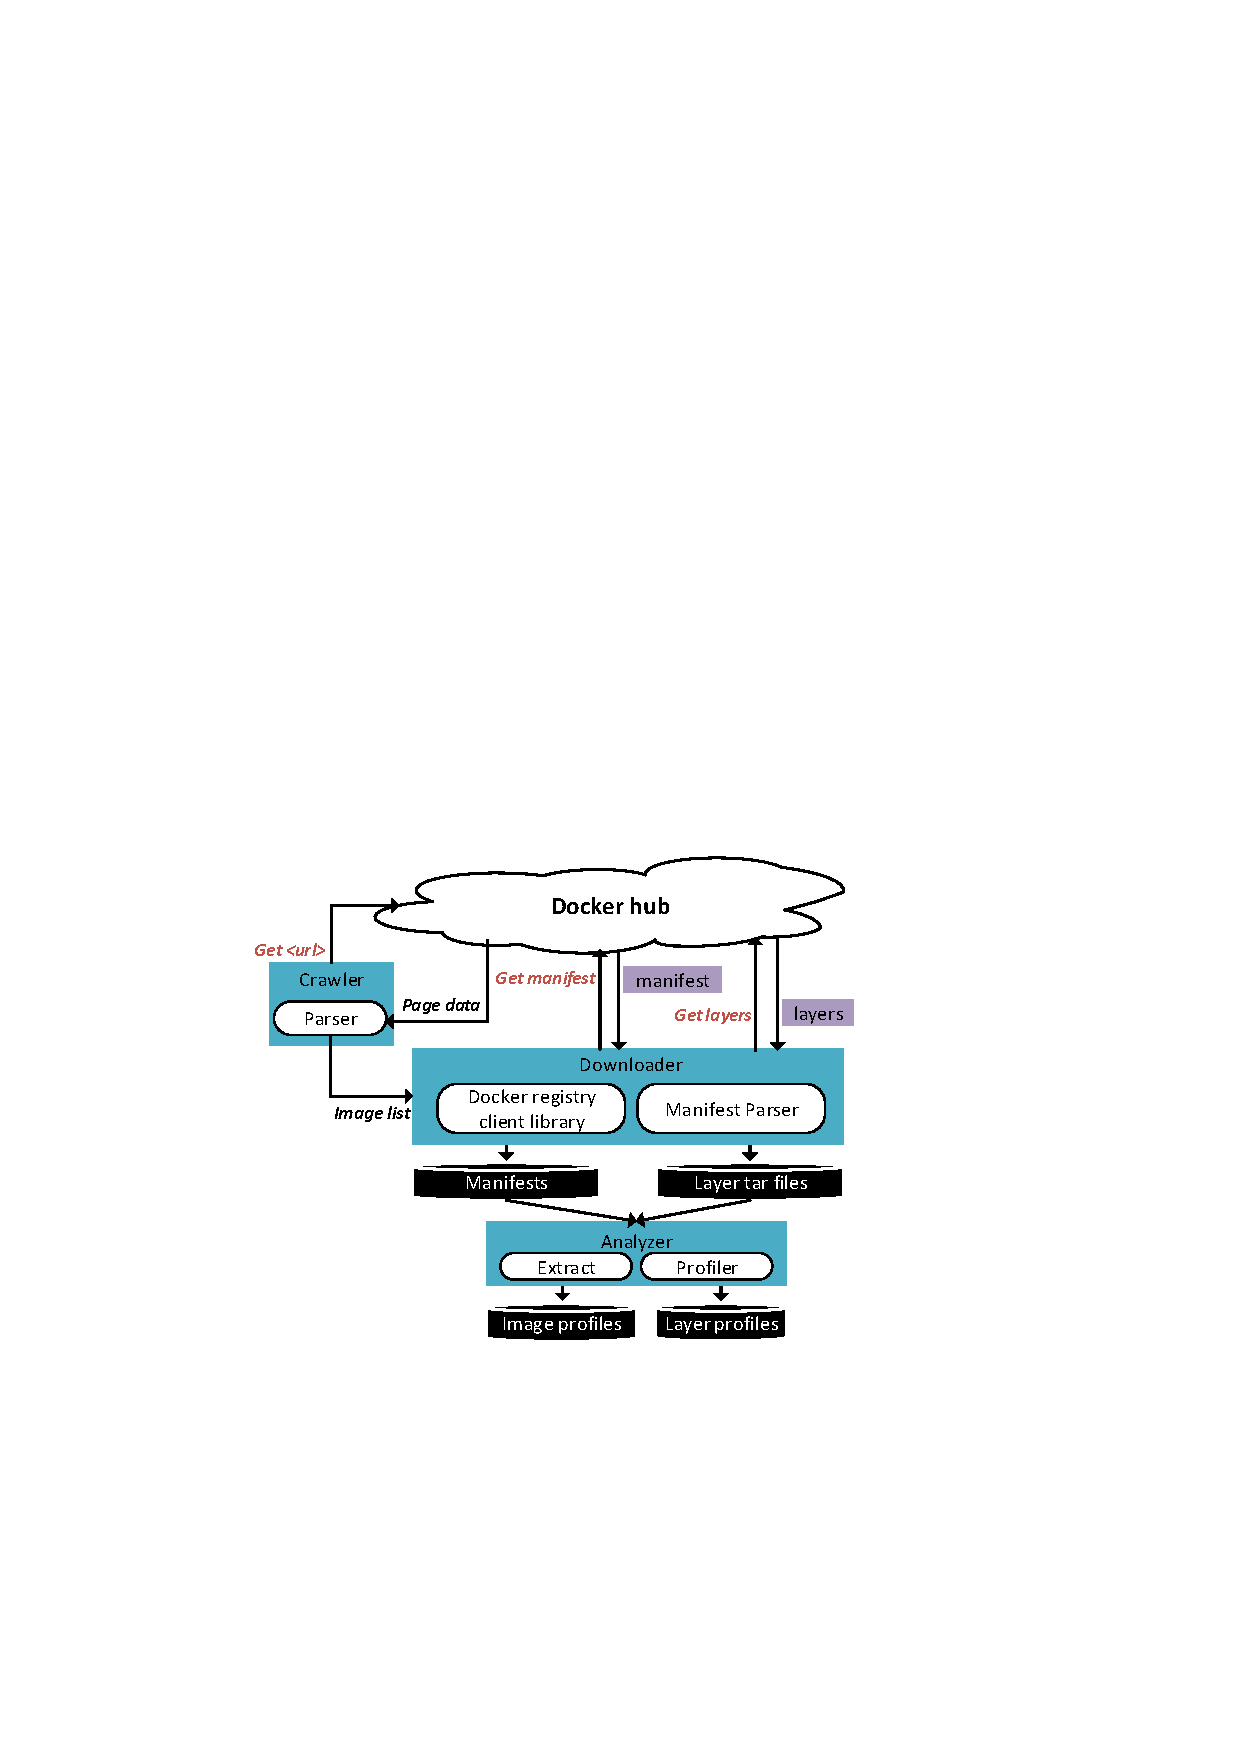
\includegraphics[width=0.5\textwidth]{graphs/fig-downloader-analyzer.pdf}\\
	\caption{Crawler, Downloader, and Analyzer
		%\vcomment{Can we add colors to this figure? Also, increase the font a bit.}
	}
	\label{fig-downloader-analyzer}
\end{figure}

\subsection{Dataset acquisition}
\label{sec:crawler}

We chose Docker Hub~\cite{docker-hub} to download a representative dataset
because (1) Docker Hub is a popular Docker registry for developers to store and
distribute Docker images, and (2) Docker Hub contains a large amount of
\emph{public} Docker images that are available for developers to download for
free.
%
We believe Docker Hub dataset is representative of other registry deployments.

To download a representative dataset from Docker Hub, web crawling is needed
because Docker Hub does not provide an API to retrieve all repository names.
%
Specifically, there are two steps: i)~crawl Docker Hub web pages to list all
repositories; ii)~download the \textit{latest} image (and referenced layers)
from each repository based on the crawler results.
%
Here, we chose latest image from each repository because (1)~the ``latest''
version is usually the newest, stable, and commonly pulled by developers;
(2)~downloading only the ``latest'' version can shorten our downloading process
since the latest images already took about 30 days to download.
%
We plan to extend our analysis to other, non-``latest'', images in the future.

\paragraph{Web crawler}

Public repositories in Docker Hub are divided into official
repositories---served by the Docker Hub partners---and non-official
repositories---provided by regular users and third-party organizations.
%
The number official repositories is less than 200, while, the majority of
repositories in Docker Hub are non-official (over 400 thousand).
%
To list non-official repositories, our crawler utilizes the Docker Hub
web-based search engine to find all available repositories.
%
As the name of non-official repositories is comprised of the user name and the
repository name separated by a ``/'', we can search for ``/'' and obtain a list
of all non-official repositories.
%
The Crawler downloads all pages from the search results and parses the web
content to build a list of all non-official repositories.
%
We ran the crawler on May 30th, 2017 and it produced a list of 634,412
repositories.
%
After removing duplicate entries (introduced by Docker Hub indexing logic), the
final repository list consists of 457,627 distinct repositories.

\paragraph{Downloader}

Instead of using the Docker client to download images, we implement our own
downloader, which calls the Docker registry API
directly~\cite{dockerregistryclient} to download manifests and image layers in
parallel.
%
Our downloader runs significantly faster than a \texttt{docker pull}-based
downloader because the latter one performs other operations besides downloading
the image, such as unpacking the layers and creating the corresponding
read-only snapshots.
%
Our downloader can download multiple images simultaneously and fetch the
individual layers of an image in parallel.
%
Layers are transferred as gzip compressed tar archives.
%
Overall, we downloaded 51~TB of data in 355,319 image manifests with 1,792,609
compressed layers. A total of 111,384 images could not be downloaded mainly because they did not have the \texttt{latest} tag. 
%
\vcomment{Say just one sentence why we did not download some images.}\nancomment{Addressed}
%
Table~\ref{tab-dataset-summary} summarizes the properties of the downloaded
dataset.

%We released both the software that we designed
%to download the images and all profiles we generated
%publicly at {\small{\url{https://elided.for.review}}}.

\subsection{Dataset analysis}

To characterize the dataset perform its redundancy analysis, we first created a
profile for each layer and image, then we performed an in-depth analysis by
using Spark~\vcomment{cite}.

\paragraph{Profiler}

For each image and each layer, profiler creates a profile in JSON format.
%
An image profile contains layer IDs, compressed size, archival size, and
compression ratio of image or layer\vcomment{what?}\nancomment{addressed}.
%
To generate a layer profile, profiler first unpacks layer tarball.
%
A layer profile consists of: (1)~layer metadata, such as layer id, compressed
size, archival size, compression ratio, directory count and file count.
%
(2)~for every file in a layer---file name, file content digest, file type, and
file size.\nancomment{add digest algori, type migic library}
%
Totally, we 1,762,639 layer profiles and 355,196 image profiles. A total of 11,130 images cannot be analyzed because their layers reported reported errors during
extraction and could not be analyzed.
%
\vcomment{Explain briefly why we did not analyze all downloaded images and
layers.}\nancomment{addressed}

\paragraph{Spark-based analyzer}

To quickly perform analysis on hundreds of thousands of profiles, we built an
8-nodes HDFS~\vcomment{cite} and Spark~\vcomment{cite} cluster.
%
We stored all the layer and image profiles in HDFS as parquet
files~\vcommnet{cite}.
%
We then performed basic and redundancy analysis using Spark SQL
module~\vcomment{cite}.
%
For example, for deduplication analysis, we first query unique file content
digests and redundant file content digests along with their repeat counts and
sizes from the layer and image parquet tables.
%
We then calculate corresponding deduplication ratios, as detailed in
Section~\vcomment{ref}.

%and investigated the following questions (RQs):  

%\paragraph{RQ1: What are the redundant ratio of layers and images?}
%
%
%\paragraph{RQ2: What are the redundant files \& why there are so many redundant files?}
%%\nancomment{how to get file type?}
%
%\paragraph{RQ3: How to reduce the redundant files?}
%\nancomment{how to prototype?}

%%%%%%%%%%%%%%%%%%%%%%%%%%%%%%%%%%%%%%%%%%%%%%%%%%%%%%%%%%%%%%%%%%%%%%%%%%%%%%
%                                                                            %
%                                OLD METHO                                   %
%                                                                            %
%%%%%%%%%%%%%%%%%%%%%%%%%%%%%%%%%%%%%%%%%%%%%%%%%%%%%%%%%%%%%%%%%%%%%%%%%%%%%%
%%\nancomment{
%%	TODO: \\
%%	1. Complete fig and table\\
%%}
%
%\lrcomment{ I think in general it would be good if we emphasize in this section, what
%was challenging about downloading all this data and how the presented approach
%overcame these challenges. \nancomment{challenges include: 1. obtaining a list of all the repositories in docker hub; 2. effectively downloading all the images. 3. indept analysis}}
%
%Our methodology consists of three steps~(Figure~\ref{fig-downloader-analyzer}):
%1)~crawl Docker Hub to list all official and nonofficial repositories;
%2)~download the latest image (and referenced layers) from each repository based
%on the crawler results; 3) unpack and analyze images and layers.
%
%%
%%
%%The first step is to massively download the Docker images from Docker registry.
%%
%%When the images are downloaded, we analyze them and calculate statistics distribution for
%%different metrics.
%%
%%The details of each step are covered in the following sections.
%%
%%\vcomment{I suggest to restructure this section simirarly to background to
%%revolve around the figure. Once you add the diagram describing our methodology
%%(like we put on the whiteboard ones), start describing components on it in the
%%order they are used: crawler, downloader, analyzer. Having two subsection:
%%``downloader'' and ``downloading images'' is confusing.
%%
%%We might want to have less deep structure also:
%%
%%3. Methodology
%%  (Figure)
%%3.1 Crawler
%%3.2 Downloader
%%3.3 Analyzer
%%}
%%
%%\nancomment{addressed}
%
%%\nancomment{
%%	figures are stored in google drive, the link is pinned in slacker;
%%	%https://drive.google.com/open?id=0B4jePsYXW6SSTTRLb0FHVXVjNUk
%%	figures/fig-docker-architecture.pdf}\\
%
%
\begin{figure}
	\centering
	% Requires \usepackage{graphicx}
	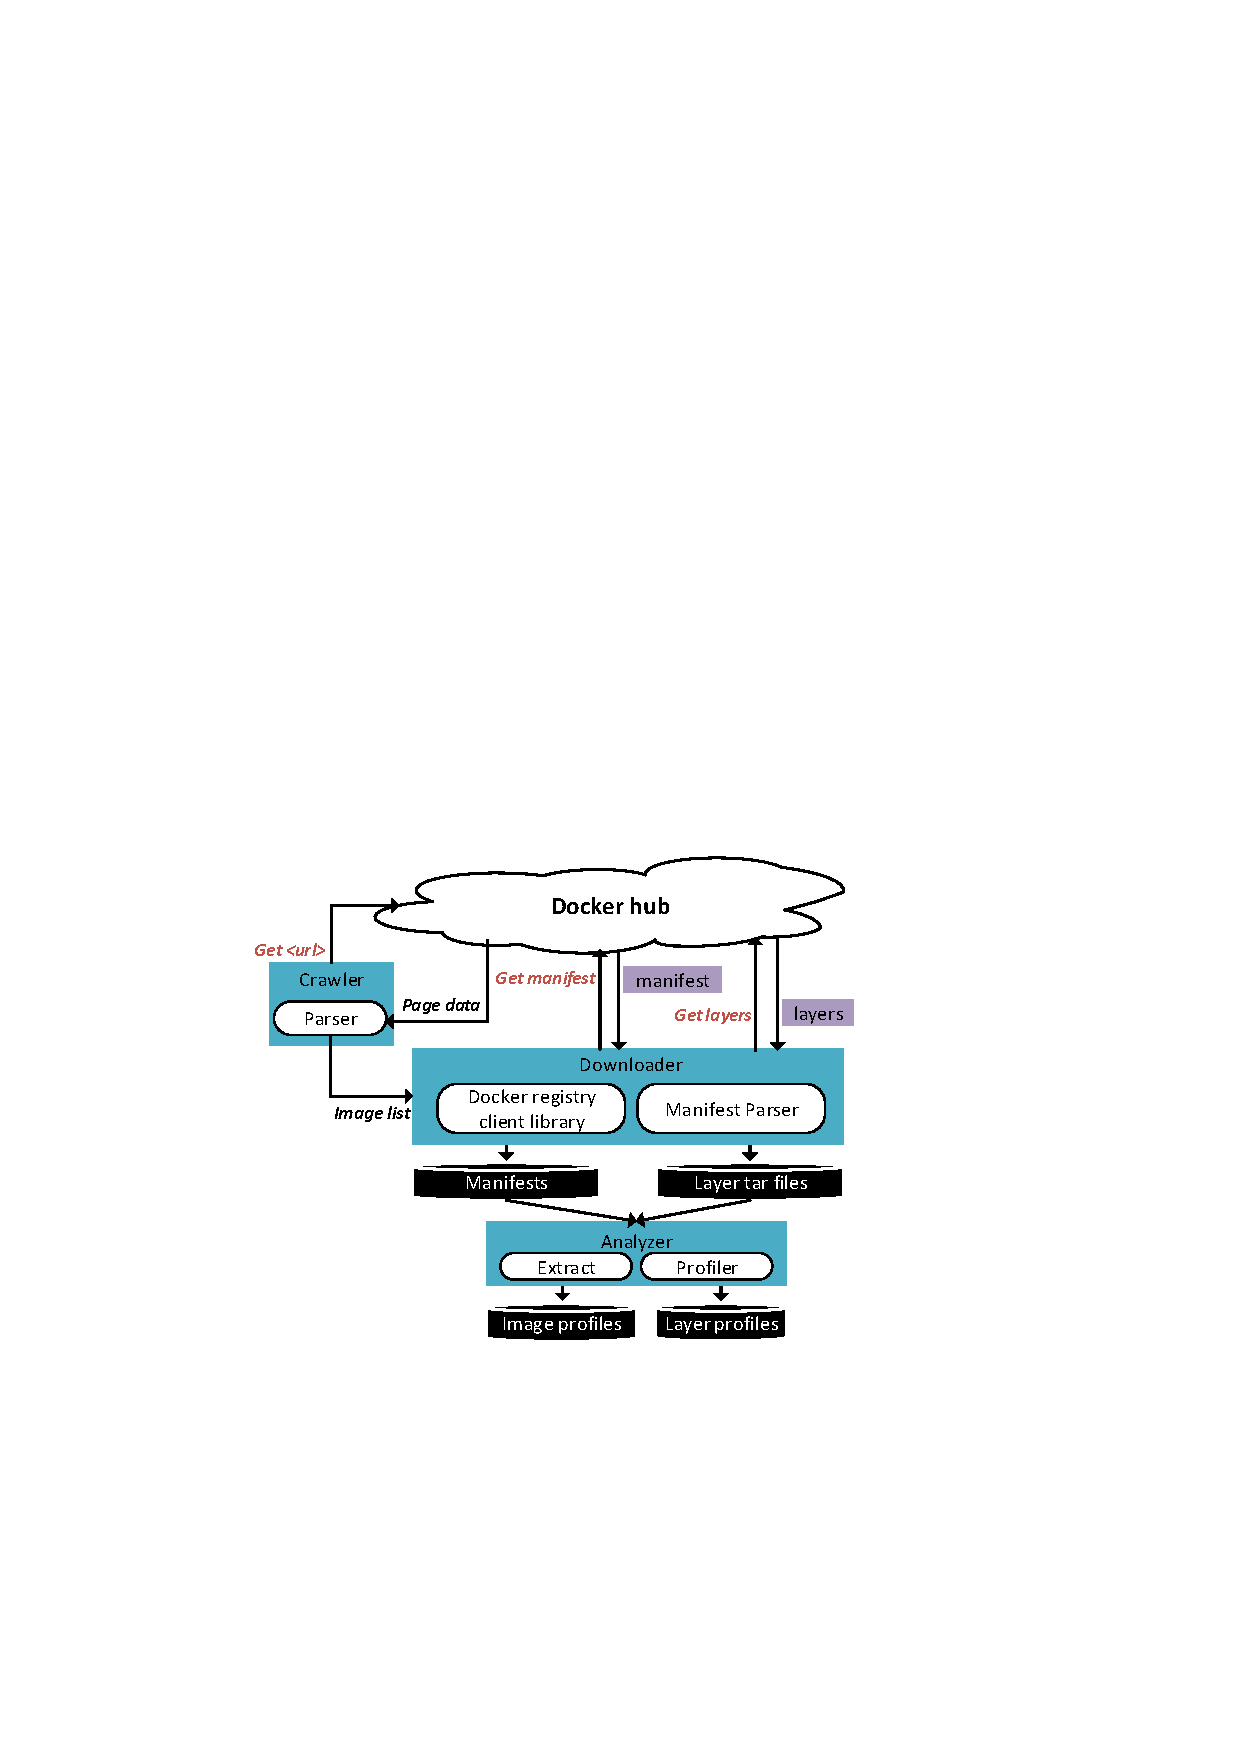
\includegraphics[width=0.5\textwidth]{graphs/fig-downloader-analyzer.pdf}\\
	\caption{Crawler, Downloader, and Analyzer
		%\vcomment{Can we add colors to this figure? Also, increase the font a bit.}
	}
	\label{fig-downloader-analyzer}
\end{figure}
%
%%how container deameon.
%%
%\subsection{Crawler}
%\label{sec:crawler}
%
%%
%To download a particular image, %or set of images (i.e., a repository)
%the name of the repository name which the image belongs to should be provided.
%The crawler is responsible
%for generating a list of repositories for the downloader.
%%as mentioned in Section~\ref{sec:docker-registry}. 
%%
%%
%%
%%\vcomment{Here and in the whole text we need to be very carefull distinguishing names 
%%of repository and image. Also discussion on image tags is missing, should be in
%%background section.}
%%\nancomment{addressed.}
%%
%Public repositories in Docker registry are divided into official
%repositories---served by the Docker Hub's partners---and non-official
%repositories---provided
%by regular users and third-party organizations.
%%, where For example, official repository Ubuntu Here is an example of the shared 
%%repository official repository Ubuntu and one of its tags. 
%%
%%A repository is a set of Docker images. A repository can be shared by pushing it to a
%%registry server. 
%%Public repositories in Docker registry can be divided into official images and non-official 
%%images.
%%
%The number official repositories is less than 200,
%% The list of official repositories
%%can be retrieved via \lrcomment{add how to list official repos}
%while, the majority
%of repositories in Docker Hub (about 400 thousands)
%are non-official.
%% (around \lrcomment{add number}).
%Listing non-official repositories requires web crawling because
%%to the best of our knowledge,
%Docker Hub does not provide an API to retrieve all repository names.
%
%Therefore, we implemented a Crawler to crawl Docker Hub and list all non-official
%repositories.
%%
%Docker Hub provides a search engine which indexes public repositories and allows
%users to search for a repository according to
%some search string. 
%%
%As the name of non-official repositories is comprised
%of the user name and the repository name separated by a ``/'',
%we can search for ``/'' and obtain a list of all non-official
%repositories.
%%``$\langle namespace\rangle/\langle repository name \rangle $", where~\textit{namespace}
%%is the user name. 
%%
%%In this case, we search for `/' and obtain a list of repositories which contains '/'.
%%
%%In other words, this method lists all the non-official public repositories in Docker Hub.
%%
%The Crawler downloads all pages from the search result.
%%
%Once web pages are downloaded, it parses the web content to build a list of
%all non-official repositories.
%
%%\lrcomment{It may be good to discuss how accurate this method is. Can we miss anything?
%%Can we get wrong results?}
%
%
%
%We ran the crawler on May 30th, 2017 and it delivered a list of 634,412 repositories.
%%
%However, the obtained list contained duplicate entries because 
%the crawling process is not atomic and some repositories have ``/'' in their description.
%%
%After removing all duplicates, the final repository list consists of 457,627
%distinct repositories. 
%%
%
%
%%
%%\vcomment{Explain why, state that it is future work.} 
%%\nancomment{addressed}
%%
%%\vcomment{I'd comment out discussion on '*'---it has low importance.}
%%\nancomment{addressed. let's comment it now and see how to deal with this issue}
%%Note that the namespace of official images is `\textit{library}'.
%%
%
%\subsection{Downloader}
%\label{sec:downloader}
%
%Docker repository is a set of images labeled with \emph{version tags}.
%%The different images in the repository are labeled with tags.
%%
%For example, \texttt{ubuntu:17.10} refers to image version \texttt{17.10} in the
%\texttt{ubuntu} repository.
%%
%If user does not provide a tag when pulling an image, 
%Docker daemon uses the \texttt{:latest} tag by default.
%For example, \texttt{docker pull ubuntu} command pulls the
%\texttt{ubuntu:latest} image.
%%
%In this work we only download images with the \texttt{:latest} tag to
%make the analysis more feasible.  We believe that the latest
%images versions represent most up-to-date state of  Docker images
%%
%and plan to analyze images with other tags in the future.
%
%
%
%%The downloader takes the list from the crawler as an input and retrieves
%%all the listed images from Docker Hub (see Figure~\ref{fig-downloader-analyzer}).
%%
%Instead of using Docker CLI to download images,
%%via the Docker Engine,
%we wrote our own downloader that calls Docker registry API directly.
%We used Docker registry client~\vcomment{insert the name, \nancomment{it is called Docker registry client}} library~\cite{dockerregistryclient} to simultaneously
%download \emph{original} manifests and image layers. \lrcomment{What does
%`original' mean here? \nancomment{without any modification}}
%%
%%\vcomment{Should we mention and cite the library that we used here?}
%%
%%\nancomment{addressed (cited in the following para)}
%%
%%
%%We decided to implement a separate downloader due to several reasons:
%%
%Our downloader runs significantly
%faster than \texttt{docker pull}-based downloader
%because the latter one performs
%operations other than downloading the
%image.
%%such as extracting
%%tar archive files and converting manifest version. 
%%
%For example, it automatically extracts each layer's tar archive file
%and creates corresponding read-only snapshot with  configured Docker storage driver.
%%and converts the manifests that are schema version 1 to schema version 2
%%(starting from Docker engine version 1.10).
%This
%not only takes considerable amount of time but also leads
%to overly high storage space utilization.
%%
%% affects
%%our results about manifest version statistics;
%%
%Furthermore, the local storage format of Docker client makes it difficult
%to analyze the contents of each layer separately.
%%Second, layer content directories are not visible for some Docker storage
%%drivers, e.g., devicemapper, which is not feasible to analyze the layer
%%content. 
%%
%%\vcomment{I think most importantly it is faster because we do not need to
%%perform extra steps that Docker client performs.}
%%\nancomment{addressed}
%%
%
%Our downloader can download multiple images simultaneously and fetch
%the individual layers of an image in parallel.
%%within each image downloading process, layers are downloaded in parallel.
%%
%%To download the original manifests and layers from Docker Hub, downloader
%%embeds a library called Docker registry client API citeXXX which only encapsulates
%%manifest and layer downloading functions in Docker engine without extracting layer
%%tarball and converting manifest version. 
%%
%%
%%\subsubsection{Downloading images}
%%
%%\vcomment{definitely need to merge this subsection with Downloader subsection.
%%See my comment for the whole section.}
%%\nancomment{addressed}
%%
%%As shown in Figure~\ref{fig-downloader-analyzer}, downloader first obtains a 
%%list of public images through crawling Docker Hub.
%%
%%Then, it starts downloading process.
%%
%%It mainly downloads two components: manifest and individual layer files. 
%The process consists of two steps.
%%
%First, fetching the manifest by sending a \texttt{GET} request to
%$/v2/\langle name \rangle/manifests/\langle reference \rangle$,
%where~\textit{name} refers to
%$\langle namespace\rangle/\langle repository name \rangle$
%and \textit{reference} is typically a version $\langle tag \rangle$.
%%
%%
%%\lrcomment{Are the following 4 sentences needed?}
%%Note that the~\textit{namespace} of official is~\textit{library}.
%%
%%The reference can include a tag or digest.
%%
%%Note that currently we only downloaded the images with~\textit{latest} tag to shorten
%%the downloading process. In the future, we will download all the images with different tags.
%%
%%As discussed in Section~\ref{xxx}, manifest consist of multiple layer digests.
%%
%%Note that Schema 2 versioned manifest also contains a config file digest.
%%\vcomment{I believe we never explained what is config file. We need to discuss in
%%in background section.}
%%\lrcomment{Do we use config files in the analysis? If they contain the command
%%to run in the container, I think that could give us some interesting insights into
%%how people use containers.}
%%
%Second, once the manifest is downloaded, the downloader uses the layer digests to
%download individual layers
%%(including the config file for Schema 2 versioned manifest)
%by sending $GET$ request to $/v2/\langle name \rangle/blobs/\langle digest \rangle$.
%\textit{Name}, as for manifests,
%refers to $\langle namespace\rangle/\langle repository name \rangle$
%while~\textit{digest} refers to the layer digest.
%%or config file digest.
%Layers are transferred as gzip compressed tar archives.
%%\vcomment{What compression is used?}
%%\nancomment{addressed}
%
%%
%%\vcomment{I believe different parts of this section belong to different
%%	earlier parts: some to crawler, some to downloader.}
%%\nancomment{addressed}
%%
%
%
%The whole downloading process took around 30 days.
%%
%Overall, we downloaded 51~TB of data in 355,319 image manifests with 1,792,609
%compressed layers.
%%
%A total of 111,384 images could not be downloaded due to three reasons.
%%
%First, 5\% of the images required authentication and
%second, 87\% of the images did not have the \texttt{latest} tag.
%Third, 8\% of the images contains layers that cannot be downloaded.
%% 0.05189255189	0.8666056166 0.0815018315
%%As we discussed in Section~\ref{sec:crawler}, we only downloaded the \texttt{latest}
%%version of an image to shorten the downloading process.
%Table~\ref{tab-dataset-summary} summarizes the properties of downloaded
%dataset.
%
%%\nancomment{2. TODO: add a table discribe:\\
%%	how many images, duplicate ratio\\
%%	how many cannot download, (removed, no latest)\\
%%	how many layers, config, manifest\\
%%	dataset}
%
%%\subsubsection{Docker image dataset statistics}
%
%
%
%%The reason probably is that Docker Hub adjusted websites'order or modified the
%%websites because of the increasing of Docker images during our crawling process.
%%Our crawler has a unavoidable delay between each HTTP requst and HTTP response. 
%%So it couldn't reflect the websites'order or website content changes. Another
%%reason is that search engine lists duplicated images 
%
%%Overall, we downloaded XXX image with XXX layers. Table~\ref{XXX} summaries
%%the statistics of Docker image dataset we downloaded. Then, we profiled the
%%layers, config files, and manifests we downloaded and calculated the statistic
%%distribution for different metrics. 
%
%%Some embedded literal typset code might 
%%look like the following :
%%
%%{\tt \small
%%\begin{verbatim}
%%int wrap_fact(ClientData clientData,
%%              Tcl_Interp *interp,
%%              int argc, char *argv[]) {
%%    int result;
%%    int arg0;
%%    if (argc != 2) {
%%        interp->result = "wrong # args";
%%        return TCL_ERROR;
%%    }
%%    arg0 = atoi(argv[1]);
%%    result = fact(arg0);
%%    sprintf(interp->result,"%d",result);
%%    return TCL_OK;
%%}
%%\end{verbatim}
%%}
%%
%%Now we're going to cite somebody.  Watch for the cite tag.
%%Here it comes~\cite{Chaum1981,Diffie1976}.  The tilde character (\~{})
%%in the source means a non-breaking space.  This way, your reference will
%%always be attached to the word that preceded it, instead of going to the
%%next line.
%
%\begin{table*}
%	\centering
%	\caption{Dataset summary} \label{tab-dataset-summary}
%	\begin{tabular}{c|c|c|c|c|c|c}%p{0.14\textwidth}
%		\hline
%		% after \\: \hline or \cline{col1-col2} \cline{col3-col4} ...
%		Num. of images crawled & Num. of unique images    & Num. of images downloaded  & Num. of layers downloaded \\
%		\hline
%		634,412                 & 457,627                 & 346,243                    & 1,763,354  \\
%		\hline
%		Num. of images analyzed & Num. of layers analyzed & Compressed dataset size              &  Uncompressed dataset size \\
%		\hline
%		344,056                     & 1,748,089                     & 51TB                        & xxx  \\
%		\hline
%	\end{tabular}
%\end{table*}
%
%\subsection{Analyzer}
%\label{sec:analyzer}
%
%The analyzer analyzes extracts downloaded layers
%and analyzes them along with image manifests.
%It creates two types of profiles for each image:
%an image profile and individual layer profiles.
%Each profile contains different metrics for the whole image and
%its individual layers, respectively.
%Profiles are stored in JSON format.
%
%
%%
%%\vcomment{I think we do not need to discuss any metrics above, as you
%%discuss them below in corresponding subsections.}
%%\nancomment{addressed}
%%
%
%\paragraph{Layer profile.}
%
%Layers are downloaded as compressed tar archive files.
%%
%To produce the layer profile, the analyzer first decompresses and extracts each
%layer tarball to a layer directory.
%%
%Then, it recursively traverses each subdirectory and obtains
%the metadata information for each subdirectory.
%
%The layer profile contains metadata about the layer, its directories,
%and files: 
%
%\{
%layer digest; 
%Archived layer size (ALS); 
%Sum of containing file sizes (FLS); 
%Compressed layer size (CLS); 
%ALS-to-CLS (compression ratio);
%FSL-to-CLS (compression ratio);
%Directory count;
%File count;
%Layer directory depth;
%\}
%
%\{
%Directory name;
%Directory depth;
%File count;
%Directory size;
%\}
%
%\{
%File name;
%File digest;
%File type;
%File size;
%\}
%
%\begin{compactitemize}
%	\item XXX
%	\item XXX
%	\item XXX
%	\item XXX
%\end{compactitemize}
%
%%file count while directory metadata covers directory depth and size
%%and file metadata includes size and type. The full set of metrics
%%covered by the layer profile is shown in Table~\ref{xxx}.
%
%
%%Each layer profile contains
%%layer metadata information, such as layer size and file count; and
%%directory metadata information for each subdirectory, such as directory
%%depth and directory size; and file metadata information for each file,
%%such as file size and file type.
%%
%%\vcomment{I'm not sure what figure we want here. I think a table might suffice.}
%%\nancomment{addressed}
%%\nancomment{3. TODO: 
%%	add a fig: discribe all layer metadata, config metadata, and manifest metadata structure} 
%%
%%\nancomment{4. TODO: 
%%	add a table\\
%%	layer tarball format statistics, tar, compressed, non compressed\\
%%	config statistics, txt, json\\
%%	manifest statistics, txt, json}
%\vcomment{Instead of the table, let's us the itemized list above for now, \nancomment{already add table 1. and we dont need to list metrics here since we present them in results}}
%
%
%\paragraph{Image profile.}
%
%To create the image profile, the analyzer parses the manifest
%and obtains the configuration information such as OS and architecture.
%Further, once individual layers are analyzed, the analyzer can build the whole image
%profile by including pointers to its layer profiles. In total, image profile includes
%the following information:
%\{
%Image name; 
%Archived Image size (AIS); 
%Sum of containing file sizes (FIS); 
%Compressed image size (CIS); 
%ALS-to-CLS (compression ratio);
%FSL-to-CLS (compression ratio);
%Directory count;
%File count;
%\}
%
%\begin{compactitemize}
%	\item XXX
%	\item XXX
%	\item XXX
%	\item XXX
%\end{compactitemize}
%
%% image metadata information,
%%such as image pull count and layer count, and image configuration
%%information, such as OS version and architecture. All metrics
%%in the image profile are shown in Table~\ref{xxx}.
%
%%Note that schema version 2 manifests store configuration information in a
%%config file as discussed in Section~\ref{sec-image-layers}.
%%\lrcomment{I think we removed the part about different manifest versions from
%%the background, should add it back.}
%%
%%As shown in table~\ref{xxx}, \gap of manifests are Schema version 2 while the
%%rest are Schema version 1. 
%
%%
%%
%%While layer profile
%%contains layer metadata information, such as layer size and file count;
%%and directory metadata information for each subdirectory, such as directory
%%depth and directory size; and file metadata information for each file, such
%%as file size and file type.
%%
%%Table~\ref{xxx} summaries the layer archive file, config file, and manifest
%%statistics.
%
%
%%\vcomment{This section (and some other places) contain a lot of ``etc.''. The
%%general rul of thumb never to ue etc. in a scientific paper. Instead,
%%say: "e.g.,", or "for example," or "for instance"}
%%\nancomment{addressed}
%%\subsubsection{Config profile}
%

\subsection{Deduplication ratio} 
\label{sec:dedup_ratio}

%In Docker registry, layers are shared among different images to eliminate
%duplicates.  
%
%In this section, we investigate if layer-level content addressable
%is enough for Docker registry to mitigate redundancy.  
%
%Specifically, we look in
%$to the sharing rate of layers across images to calculate how much space is
%aved by using layer-level content addressable storage.  
%
%We also investigate
%that how much redundant data exists across images.

\paragraph{Layer sharing}

\begin{figure}
	\centering
	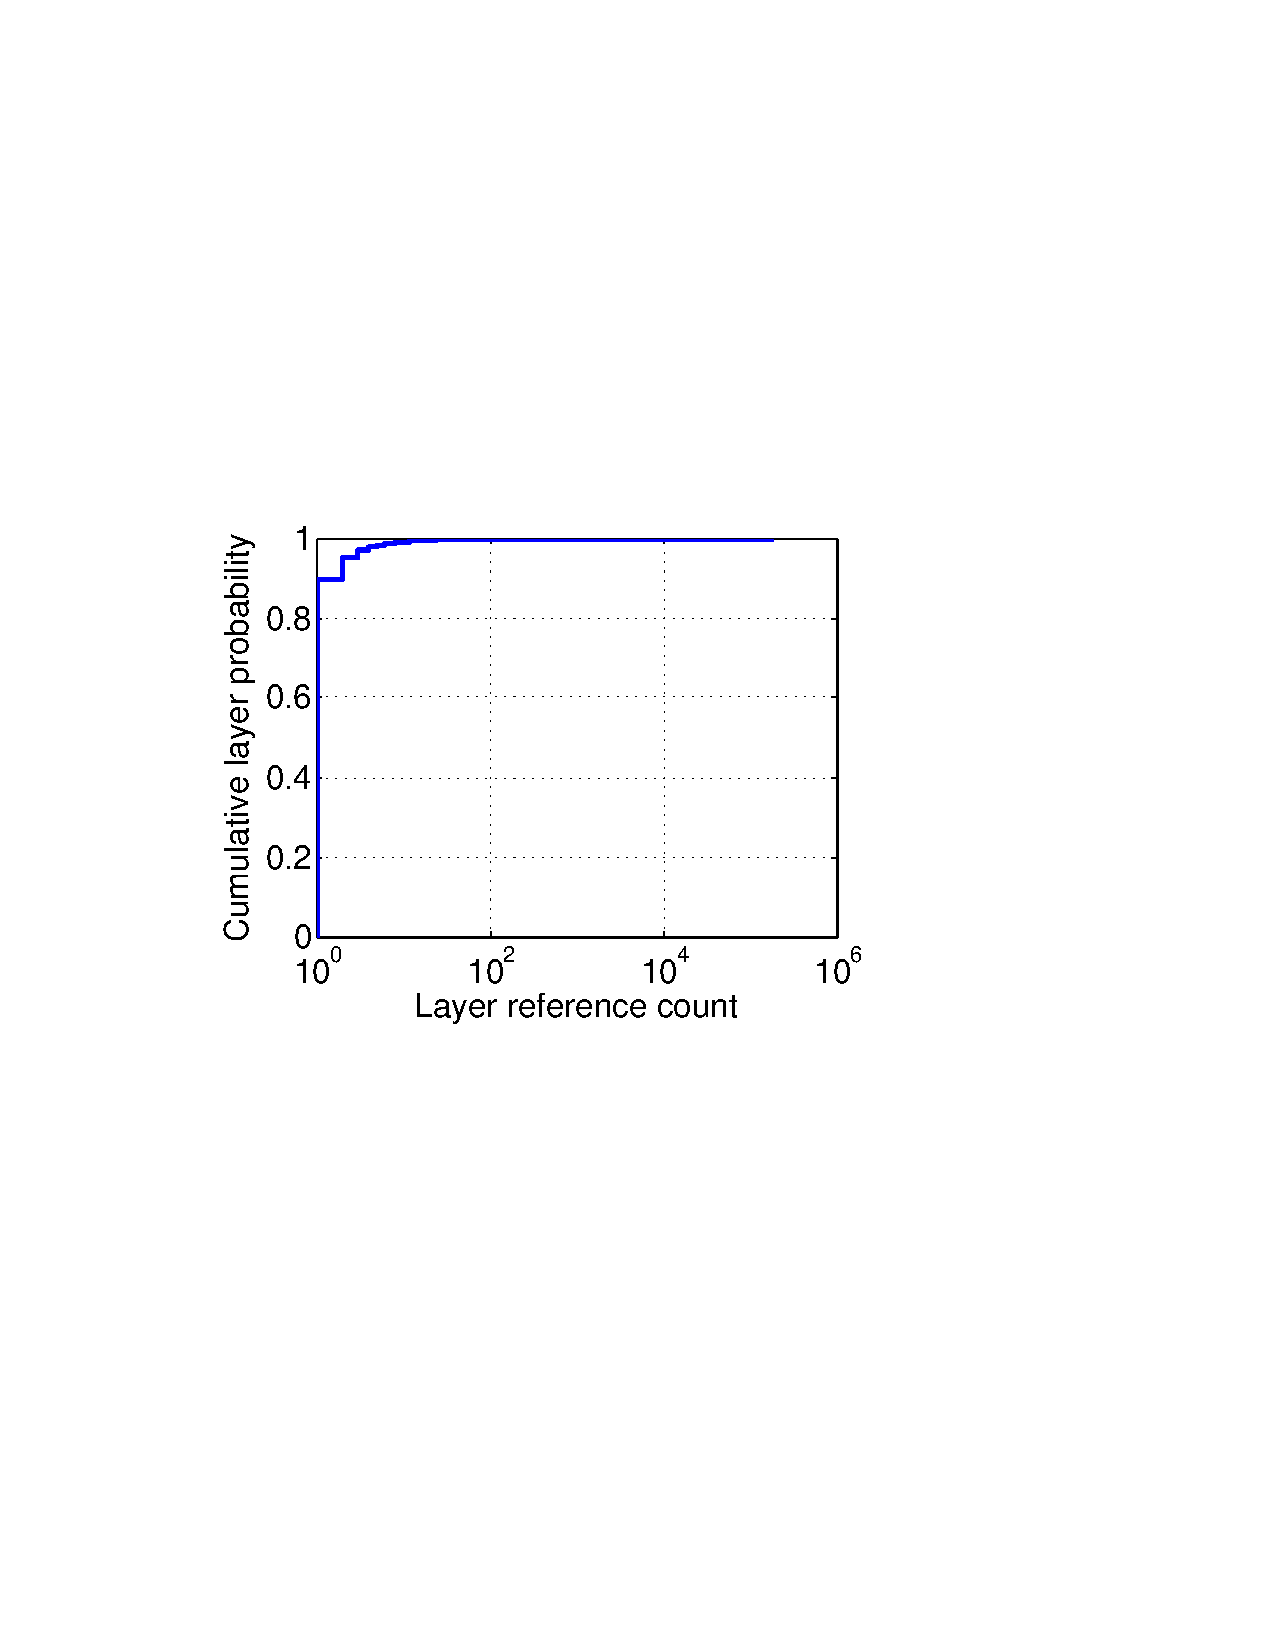
\includegraphics[width=0.21\textwidth]{graphs/shared-cnt-cdf.pdf}
	\caption{CDF of layer reference count.
	}
	\label{fig:ref_count}
\end{figure}


In its simplest implementation Docker would not support layer sharing.
%
Instead, every image would be a single flat archive.
%
In fact, some existing containerization frameworks \VT{cite singularity and
openvz} use flat images.
%
Our estimates show that without layer sharing our dataset would grow from 47TB
to 85TB, resulting in \textbf{1.8$\times$} deduplication ratio.
% 
We further computed for each layer, how many times it is referenced by images.
%
Figure~\ref{fig:ref_count} shows that around 90\% of layers are referenced by
only a single image, additional 5\% are referenced by 2 images, and less than
1\% of the layers are shared by more than 25 images.
%
%Accordingly, we calculated the total storage space consumed before layer-level
%content addressability was adopted, which was 84.75 TB.  Thus the redundant
%ratio achieved by layer-level content addressability is around 1.8.
%
%Figure~\ref{} shows the absolute values, revealing that almost 1.5 million
%images are only referenced once.  \acomment{Figure is missing} While there is
%again a large spectrum of reference counts, the maximum is 33,428, the vast
%majority of layers is not shared. 
%
%This hints that the layer-based approach to improve storage efficiency is
%barely utilized and there is room for improvement in how to construct more
%sharable layers.
%
%\emph{These findings reveal that layer level content addressable store has not
%been very successful and most of the layers that exists in Docker Hub are not
%shared among images.
%
%Hence, there is a dire need of a better redundancy management.}
%
%
Interestingly, there were xxx\% layers that were referenced about 1 million
times.
%
Our investigation showed  that these layers are~\VT{Verify this
sentence and extend with analysis.}

\VT{Use \% instead of probability in all Figures (both # and labels).}

\paragraph{Compressibility}



\paragraph{File-level deduplication}
%As discussed in compression ratio analysis, we see that there is redundant
%data in both layers and images.  We conducted simple form of deduplication to
%Interestingly,
Next, we calculate deduplication ratio in terms of file count and capacity for
the complete uncompressed dataset. %(Table~\ref{tbl:overall-redundant_ratio}).
%the redundant file overhead of the uncompressed dataset 
%
We find that majority of the files have more than one copy (99.42\%), which
take up over 89\% of capacity.
%
\VT{not clear what exactly takes 89\% of capacity}
%
After elimination of file duplicates, the percentage of such files decreases
from 99.42\% to 2.59\%.  
%
\VT{huh? Shouldn't the percentage of duplicate files go to 0?}
%
Overall, only 3.17\% (23.92 TB) of files are unique files while 96.83\% of
files (143.28 TB) are redundant copies. 
%
Correspondingly, the deduplication ratio is 96.83\% and 85.69\% in terms of
file count and capacity, respectively.
%
\VT{let's use $\times$ for dedup ratio, it's conventional}.
%
% Table~\ref{tbl:overall-redundant_ratio} summaries the overall redundant file
% overhead in terms of file count and capacity.
%
\textit{Finding 1: Majority of files in Docker registry are duplicates which
occupy most of capacity, indicating that Docker Hub has severe redundancy
problem.}

%\begin{table} 
	\centering 
	\scriptsize  
	%\begin{minipage}{.5\linewidth}
	\caption{Redundant ratio in terms of file count and capacity}
	\label{tbl:overall-redundant_ratio} 
	\begin{tabular}{|l|l|l|}%p{0.14\textwidth}
		\hline  
		& File count & Capacity \\ 
		\hline 
		Repeat cnt = 1 & 0.58\% & 10.87\%\\
		\hline 
		Repeat cnt $>$ 1 after dedup. & 2.59\% & 3.44\%\\ 
		\hline 
		Repeat cnt $>$ 1 before dedup.  & 99.42\%  & 89.13\%\\ 
		\hline 
		Unique dataset (Uncompressed) & 3.17\% (167,251,437)  &  14.31\% (23.92 TB) \\ 
		\hline 
		Total dataset (Uncompressed) & 5,278,465,130 & 167.20 TB \\ \hline 	
			%\hline 
	\end{tabular} 
\end{table} 


\VT{Move all figures to separate fig- files and tables to tab- files.}

\begin{figure} \centering
	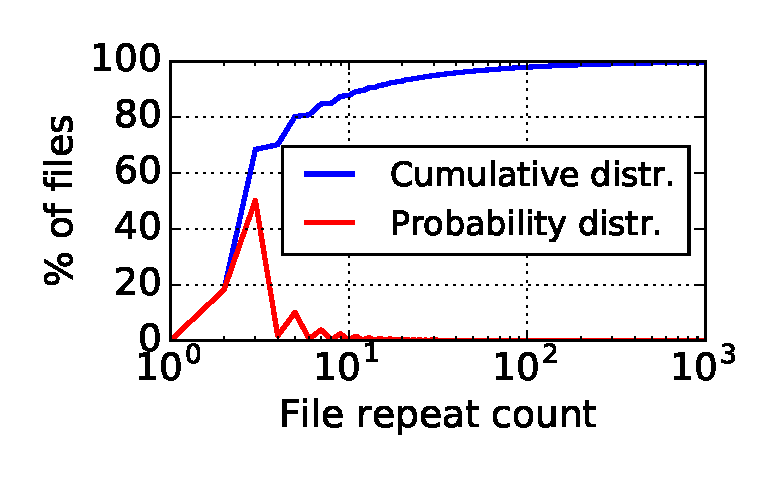
\includegraphics[width=0.45\textwidth]{graphs/File_repeat_count.eps}
	\caption{File repeat count distribution.  } \label{fig:file-repeat-cnt}
\end{figure}

We further analyzed the repeat count for for various files.
%
Figure~\ref{fig:file-repeat-cnt} shows the cumulative and probability
distribution of file repeat count.  
%
We see that over 99.42\% of files have more than one copy.
%
Around 50\% of files have 4 copies and 90\% of files have less or equal than 10
copies. 
%
The file that has the maximum repeat count---\VT{SPECIFY}---is an empty file.
%
\VT{Do we know anything about those empty files}.

\subsection{Deduplication by file types}

\begin{figure} 
	\centering
	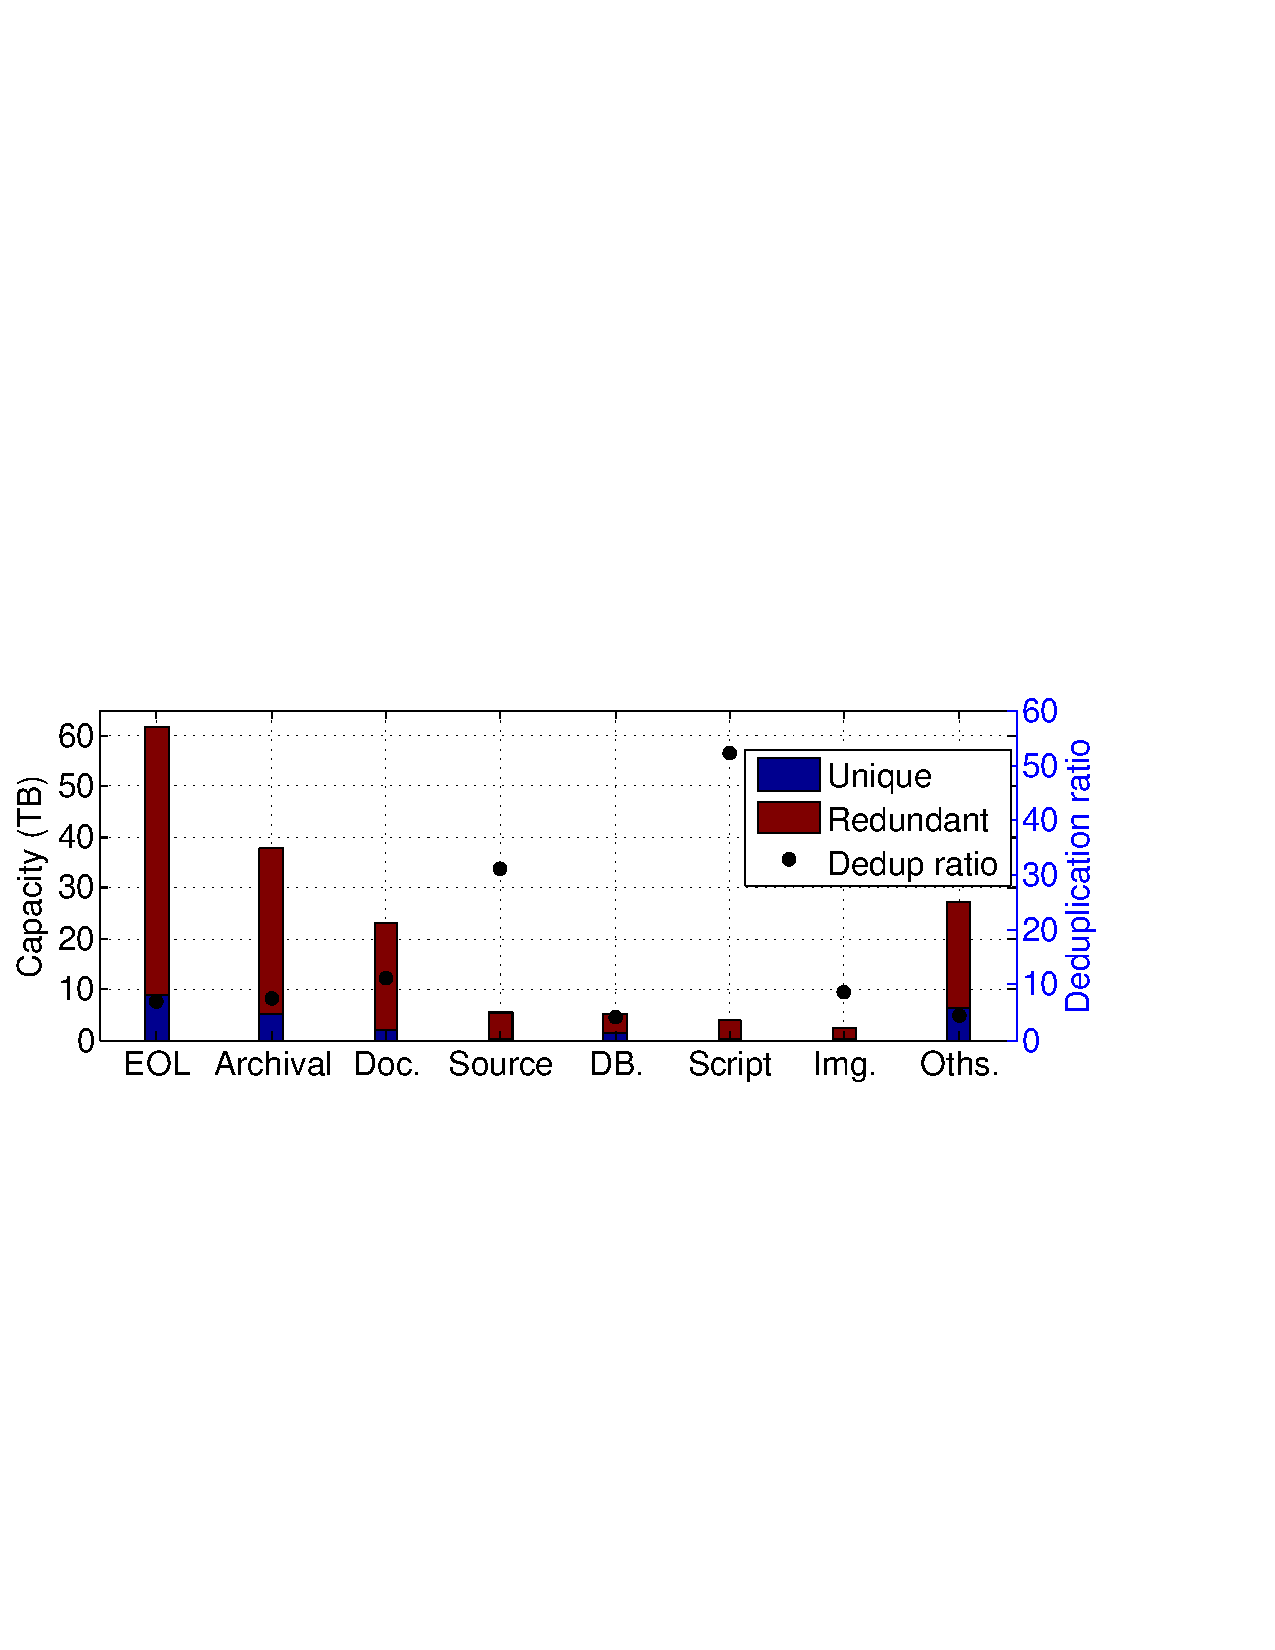
\includegraphics[width=0.45\textwidth]{graphs/dedup-overall} 
	\caption{Deduplication ratio for seven file classes---EOL, archival, documents, source code, database, scripts, images---and other files.
	Light bars indicate the original storage utilization while dark bars represent the capacity after removing redundant files.
	Dots shows the corresponding deduplication ratio.
%
%\VT{Can we stretch X axis to column width to have more space for X-axis labels?}\NZ{addressed}
%%
%\VT{Explain what blue and red bars mean here, as well as dots. Explain
%if dedup ratio is in terms of capacity or file counts.}\NZ{addressed}
%
} 
	\label{fig:dedup-overall} 
\end{figure}




To understand the sources of high data redundancy among Docker images, we
investigate deduplication for common file types.
%
We identify \VT{XXX - how many?} file types (e.g., JPG, C/C++ code, Java files)
using the file type library~\VT{\cite{XXX}} and then group file types into 7
classes by their usage scenarious:
%
1)~executables, libraries, and object files (EOL)
%
\VT{Maybe call them ``Exec.`` instead on the graph and everywhere?}
%
2)~archival,
%
2)~documents,
%
4)~source-code,
%
5)~scripts,
%
6)~images,
%
7)~database files. 
%
\VT{I'd add extensions example in parenthesis for every class. E.g., document is not intuitive.}
These classes consitute 98.4\% of the whole dataset.
%
\VT{Weird, ``Oths'' is ~30TB in the graph, so much more than 1.6\%. What's
going on?}


Figure~\ref{fig:dedup-overall} illustrates the deduplication results for these
classes.
%
The overall deduplication ratio is \textbf{6.99$\times$} and most type classes
have a comparable ratio (see dots in Figure~\ref{fig:dedup-overall}.
%
E.g., the deduplication ratio for EOL files is \textbf{7.14$\times$}.
%
However, source code, scripts, and documents exhibit significantly higher
deduplication ratio--- \textbf{31.25$\times$} for source code,
\textbf{50$\times$} for scripts, and \textbf{12.5$\times$} for documents.
%
This indicates that Docker image builders are prone to frequently replicate
source code, scripts, and documents.
%
%Moreover, the source code and script duplicates generate additional executables
%and object files that are identical.

We found that redundant C/C++ source code takes up over 77\% of the capacity
occupied by source code.
%
Looking closer we found, for example, that Google Test~\cite{googletest}---a
cross-platform C++ test framework available on GitHub~\cite{github}---is
frequently replicated.
%
\DIM{Okay - but could we say something more precise, e.g., what \% of 77\% is
taken by gtest?}
%
Interestingly, we found there are multiple Docker repositories \DIM{Docker
repositories?}\NZ{yes} related to Google Test while there is no official
repository for Google Test.
%
We suspect that many developers replicate open source code from external public
repositories, such as GitHub, and store them in containers.
%
This would also explain the shared source code across different images.
%
\VT{give few more example in addition ot Google Test}


Docker Hub allows developers to automatically build images from
source code in external public repositories and automatically push the built
image to their Docker repositories, we believe that more open source code
may be replicated into different images stored in Docker Hub registry.
%
\VT{I don't understand the last sentence. ``more'' than what?.. And who can 
replicate? don't use passive voice to make it clear.}
%
\textit{To eliminate redundant open source codes in Docker registry in the
future, we suggest that Docker Hub creates offical images for popular
open source codebases so developers can directly pull the image as a
read-only layer}.

Next, we see that EOL files, archival, and images have a similar deduplication
(around \textbf{6.99$\times$}). 
%
Compared with other type classes, the redundant EOL files and archival files
occupy over half of the capacity (51.4\%). 
%
\VT{can we same something where the duplicate archive files come from?.. (Similarly to
Google Test example)}
%
%This is mainly because EOL and archival file sizes are bigger than other type
%group.
% 
Database related files have the lowest deduplication ratio (\textbf{4.2$\times$}),
which contributes little to the overall savings.

All common file types have a high deduplication ratio.  Especially, EOL and
archival files contribute a lot to the overall savings.
%
Also, developers are likely to reuse code rather than create their own.
%
\DIM{Ffrom the data we see there is high source code dedup, but this might be
too much of a generic statement based on this data.}

%We see that 43.15\% of redundant files are documents, 
%%
%Documents have the
%largest number of redundant files (), indicating that users replicate more
%documents than other clusters. While the redundant document files only consume
%14.54\% (20.87 TB) of storage space, indicating that the size of redundant
%document files are small (10.2 KB on average). In comparison, 13.38\% and
%10.23\% of files are EOL files and source codes, which take up over 3.66\%
%(5.3 TB) and 36.85\% (52.9 TB) of redundant storage space, indicating that
%users replicate source codes and create big identical EOF files (108.6 KB on
%average).
%
%Archival files and scripts have almost similarly number of redundant files,
%8.53\% for archival and 8.69\% for scripts. However, archival cluster consumes
%more storage space than that of scripts (32.9 TB for archival and 3.9 TB for
%scripts) since archival file size (81 KB on avg.) is inherently higher than
%script size (9.4 KB on avg.).
%
%We found that 4.15\% of redundant files are image files and 0.09\% of
%redundant files are relevant to database, which takes 2.1 TB and 3.9 GB
%storage space respectively. There are 10.17\% (21.2 TB) of redundant files in
%\textit{Other} cluster which mainly contains binary data (9.76), GNU message
%catalog (3.37 TB), font related type (3.02 TB), git pack files (1.9 TB), etc. 
%
%\textit{ Finding 1: 13.38\% and 10.23\% of redundant files are source codes
%and EOL files, which take up over 3.66\% (5.3 TB) and 36.85\% (52.9 TB) of
%redundant storage space, indicating that users are more prone to replicate
%source codes and create identical big EOF files, while 43.15\% and 8.53\% of
%redundant files are documents and archival files, which account for 14.54\%
%(20.87 TB) and 22.93\% (32.9 TB) of redundant storage space, indicating users
%replicates more documents and archival files compare to other clusters.}


%
%\begin{figure} 
%	\centering
%	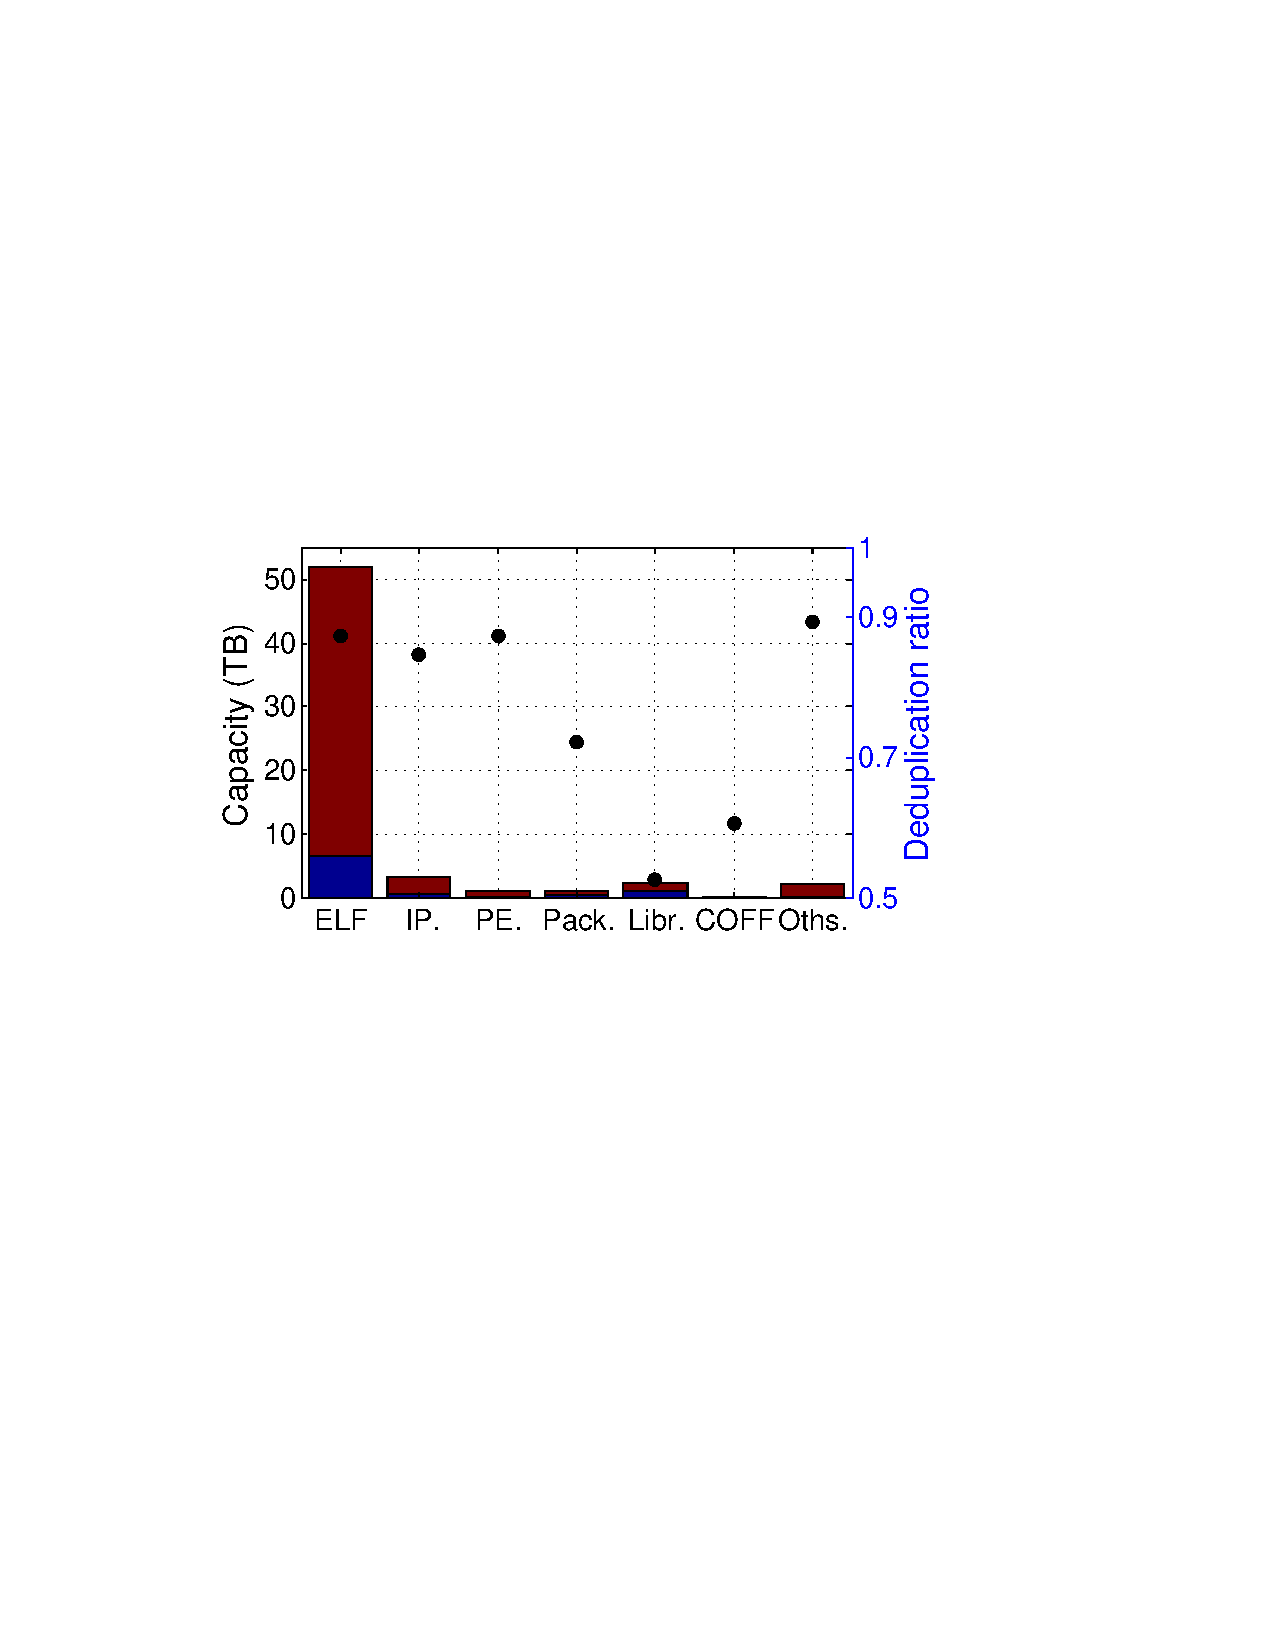
\includegraphics[width=0.35\textwidth]{graphs/dedup-eol} 
%	\caption{Deduplication results for EOL files: ELF, intermediate representation, PE32/PE32+ files, Debian/RPM binary packages, 	Libraries, COFF files.} 
%	\label{fig:dedup-eol}
%\end{figure}
%
%\paragraph{Executable, object code, and libraries (EOL)} We further calculated
%the deduplication ratio for specific file types in each common type group. 
%%
%We
%started from EOL group since it occupies the most capacity and contributes a
%lot to the overall savings after deduplication. 
%%
%Figure~\ref{fig:dedup-eol} shows the deduplication results for EOL files.  
%%
%We
%see that ELF files, intermediate representations, and PE files have the highest
%deduplication ratio (around 87\%). 
%%
%Especially, the redundant ELF files occupy
%the most capacity (73.4\%). 
%%\nancomment{replace MS exec with PE files}
%Libraries and COFF files have the lowest deduplication ratio of 53.5\% and 61\%
%respectively.
%
%We also calculated the deduplication ratio for each intermediate representation
%and libraries. 
%%
%We found that all the intermediate representations have a very
%higher deduplication ratio (greater than 77\%). 
%%
%Especially, the redundant
%Python byte-compiled codes take up to 67\% of capacity occupied by intermediate
%representations. 
%%
%Although overall library's deduplication is lower, we found
%that GUN C/C++ library and Palm OS dynamic library have a higher deduplication
%ratio over 90\%.
%
%\textit{Finding 4: ELF files have the highest deduplication ratio among all EOL
%files and contribute most to the overall savings. Python byte-compiled codes
%have the highest deduplication ratio and also achieve a better capacity savings
%after dedupliation compared with other intermediate representations. Most
%libraries have the lowest deduplication ratio among all EOL files.}
%%
%%%As shown in , intermediate compiled files have the largest number of
%%redundant copies (333,261,220, 63.7\%), which only take up to 5.3\% (2.8TB) of
%%EOL redundant storage space, indicating that users creates more small
%%redundant intermediate compiled files. Among all the intermediate compiled
%%files, python byte-compiled files have the largest number of redundant copies
%%(64.1\%, 213,753,591), which account for 79.4\% (2.2TB) of EOL redundant
%%storage space as shown in Figure~\ref{fig:type-compiled}.  % %We found that
%%there are various redundant intermediate compiled files in layers in addition
%%to Python byte-compiled, such as Erlang beam files, Xemacs/emacs compiled
%%files, compiled Java class, Mach-o fat files, Guile object bytecode, and llvm
%%bitcode files. We see that 21.6\% (71,830,155) and 10.12\% (33,740,399) of
%%redundant intermediate compiled files are terminfo compiled and compiled java
%%class files, which consume 76.4 GB and 104.4 GB storage space.   
%%
%%%ELF files have the largest redundant capacity %A large executable group is
%%ELF file type, which consists of ELF 64/32-bit LSB relocatable, shared object,
%%executable, core file, processor-specific for x86-64, MIPS, %ARM, Intel 80386,
%%etc. architectures.  %Another executable group contains VAX COFF executable,
%%PE32/PE32+ executable for Windows, and 386 pure executable, VMS Alpha, etc.
%%%\% of files are script executable, which contains python, shell, etc.  %\% of
%%files are RPM, Debian bin
%%
%%%\begin{figure} %	\centering %
%%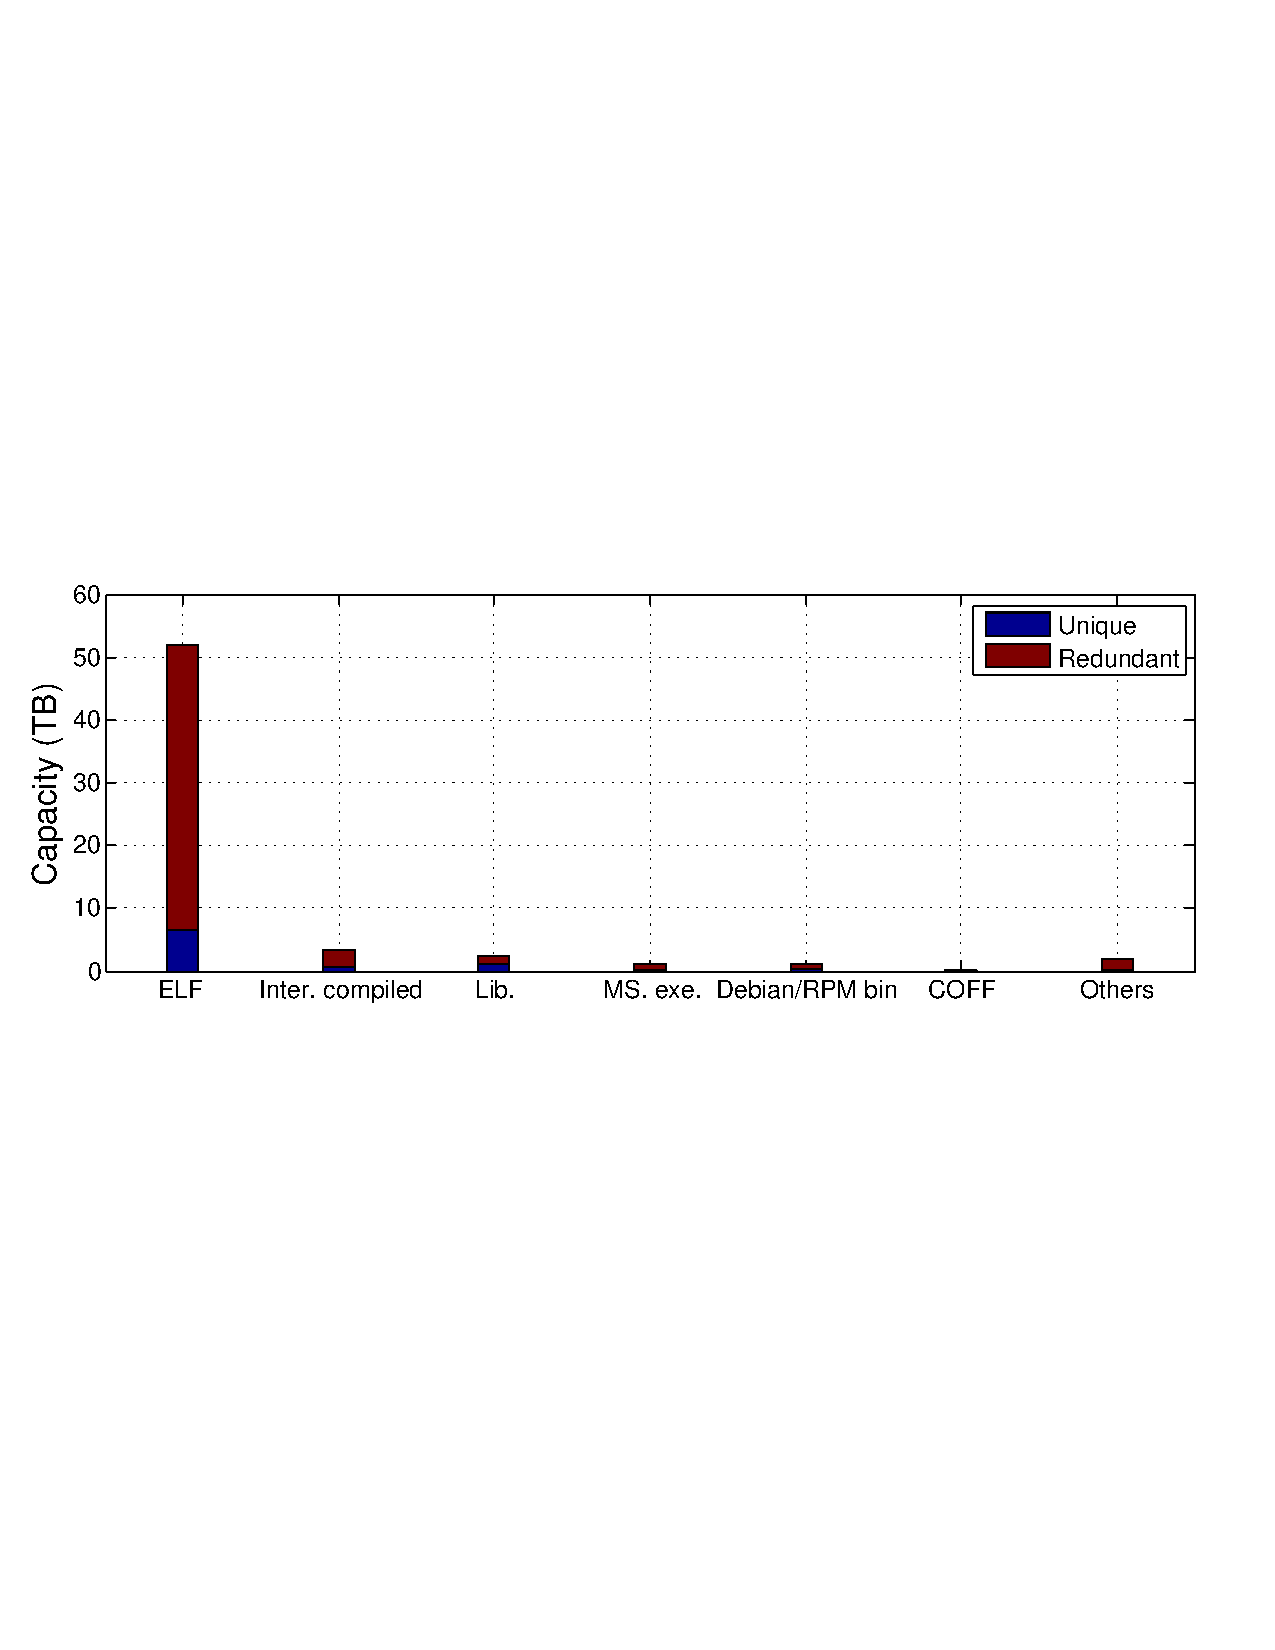
\includegraphics[width=0.5\textwidth]{graphs/type-exec-cap} %
%%\caption{\nancomment{Deduplication results for EOL files}.  %	} %
%%\label{fig:type-eol} %\end{figure}
%%
%%%Finding 2: 31.4\% (164,059,690) and 63.7\% (333,261,220) of EOL files are ELF
%%files and intermediate compiled files, which take up over 85.7\% (45.3TB) and
%%5.3\% (2.8TB) of redundant storage capacity, indicating that users replicate
%%or create more identical ELF files and intermediate compiled files. 64.1\%
%%(213,753,591) of intermediate compiled files are Python byte-compiled files,
%%which take up to 79.4\% (2.2TB) of redundant storage space, indicating that
%%users compiled more Python scripts (similar to Finding 2.)
%%
%\paragraph{Source code (SC.)}
%%
%%%Finding 3: 80.2\% (548,507,865) of source codes are C/C++ source, which take
%%up to 79.7\% (4.2TB) of redundant storage space, indicating that users are
%%more prone to duplicate C/C++ codes, which results in more ELF file replicas.
%%%The last group contains
%%
%\begin{figure} 
%	\centering
%	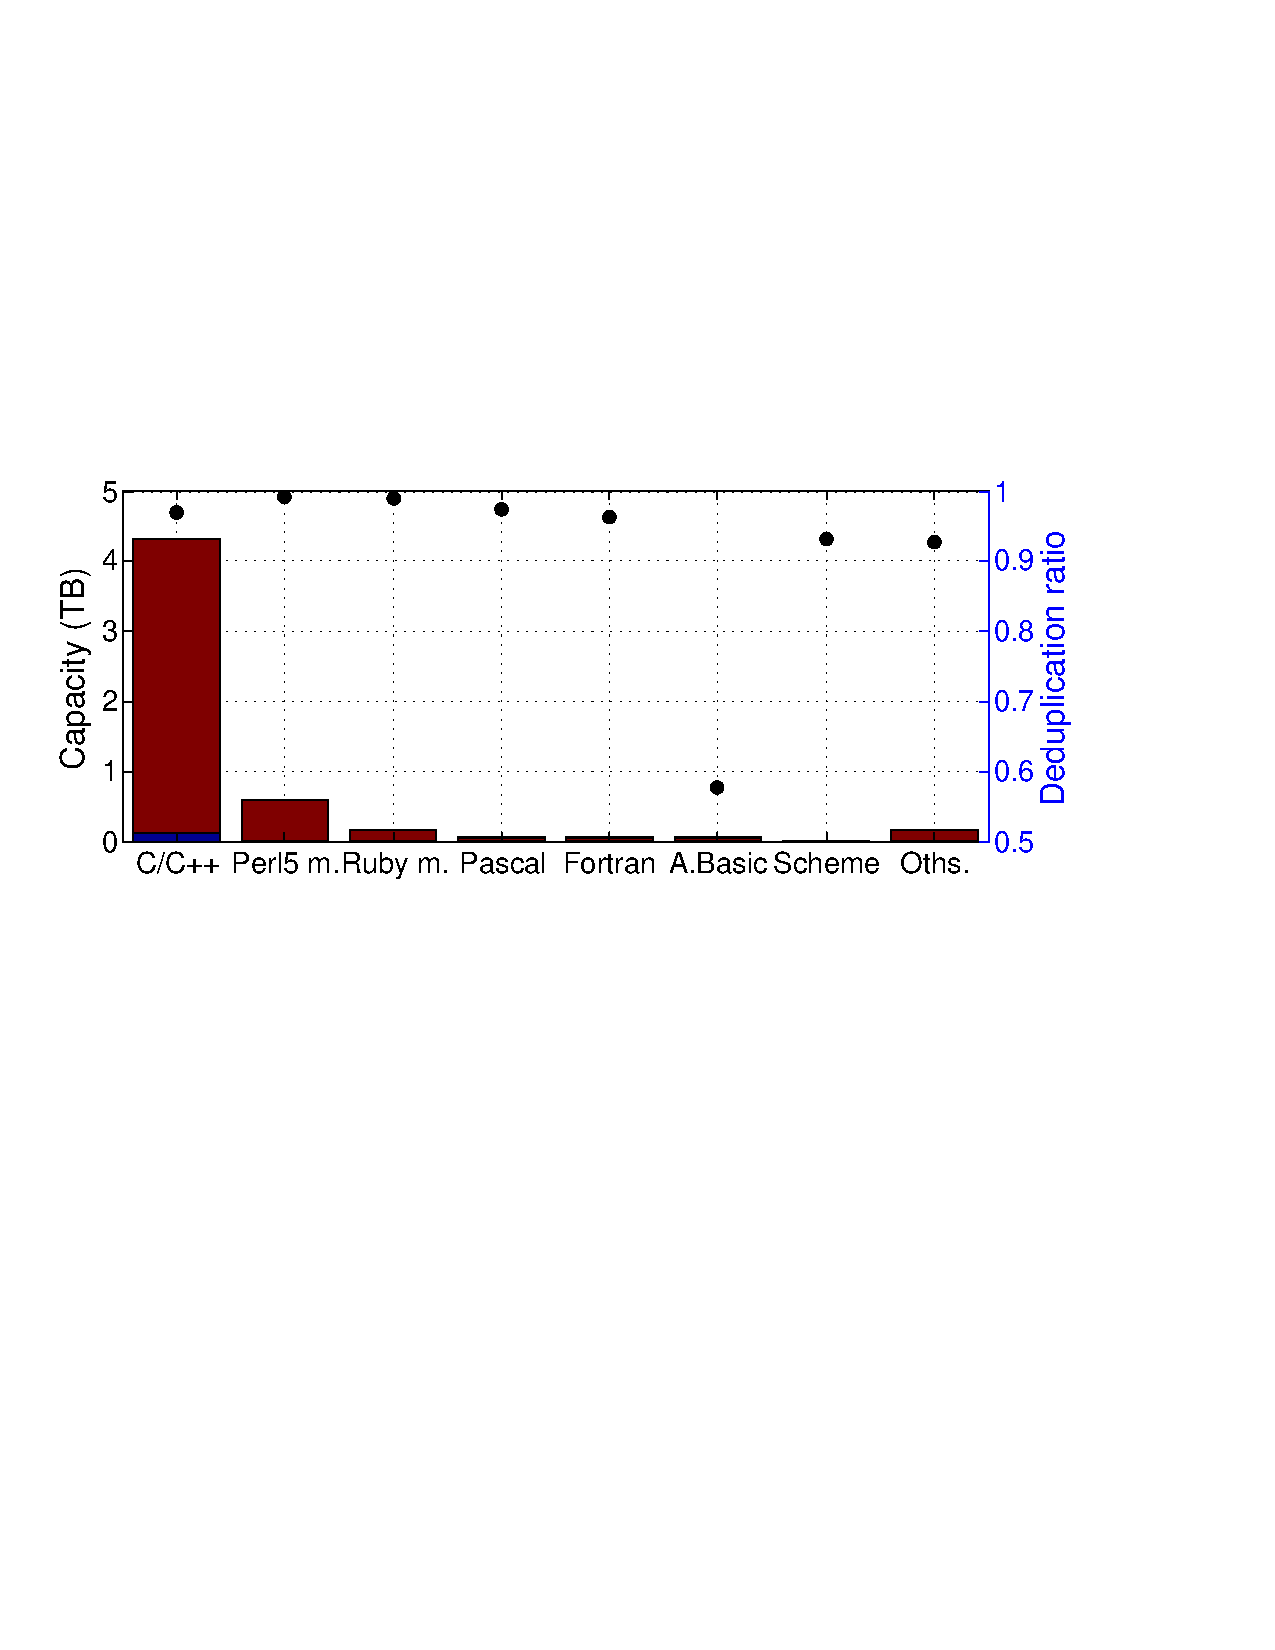
\includegraphics[width=0.35\textwidth]{graphs/dedup-sc} 
%	\caption{Deduplication results for source codes: C/C++ source, Perl5 module source, ruby module
%		source, pascal program, fortran program, Applesoft Basic program, Lisp/scheme
%		program, and other source codes.  } 
%	\label{fig:dedup-sc} 
%\end{figure}
%
%As discussed, Docker developers are more prone to replicate codes. 
%%
%To find out
%which kind of source codes are replicated frequently, we conducted
%deduplication on 7 common source codes as shown in Figure~\ref{fig:dedup-sc}.
%
%We see that all the source codes have a high deduplication ratio over 90\%
%except Lisp/scheme program. 
%%
%Especially, the redundant C/C++ source codes take
%up over 77\% of capacity occupied by source codes. 
%%
%To find out why there are so
%many C/C++ source codes, we inspect the C/C++ source codes and find a
%frequently replicated C/C++ source code called Google Test~\cite{googletest}, which is
%a cross-platform C++ test framework and available in GitHub~\cite{github}.
%%
%Interestingly, we found there are plenty of repositories related to Google Test
%while there is no official repository for Google Test. 
%%
%We suspect that many
%developers replicate open source code from external public repositories, such
%as GitHub, and store them in containers. 
%%
%This would also explain why there are
%so many shared source codes across different images. 
%%
%Docker Hub
%allows developer to automatically build images from source code in external
%public repositories and automatically push the built image to their Docker
%repositories. Thus we believe that more open source code would be replicated into
%different images stored in Docker Hub registry. 
%%
%\textit{To eliminate redundant
%open source codes in Docker registry in the future, we suggest that Docker Hub
%can create more offical images for popular open source codes so that developers
%can directly pull the image as a read-only layer. }
%
%\textit{Finding 5: C/C++ source codes have a high redundant ratio and
%contribute a lot to the overall savings. Many redundant source codes shared
%cross images are replicated or automatically build from external public
%repositories. To eliminate redundant source codes in Docker registry, we
%suggest to create more official images for these open source codes and convince
%developers to pull them from registry.}
%%
%%%\nancomment{found some libc++ source code here, did not put them into
%%libraries.} % shows the redundant file count and storage capacity distribution
%%for source code. C/C++ source codes have the largest number of redundant
%%files. 80.2\% (548,507,865) of source codes are C/C++ source, which take up to
%%79.7\% (4.2TB) of redundant storage space, indicating that users are more
%%prone to duplicate C/C++ codes, which results in more ELF file replicas.
%%
%%%We also found other source codes, such as Perl5 module source code (9.5\%),
%%ruby module source code (7.6\%), assembler source code (1.1\%), pascal source
%%(0.7\%), fortran program code (0.01\%), applesoft basic source code, and
%%Lisp/scheme source code (0.17\%).
%%
%%%\begin{figure} %	\centering %
%%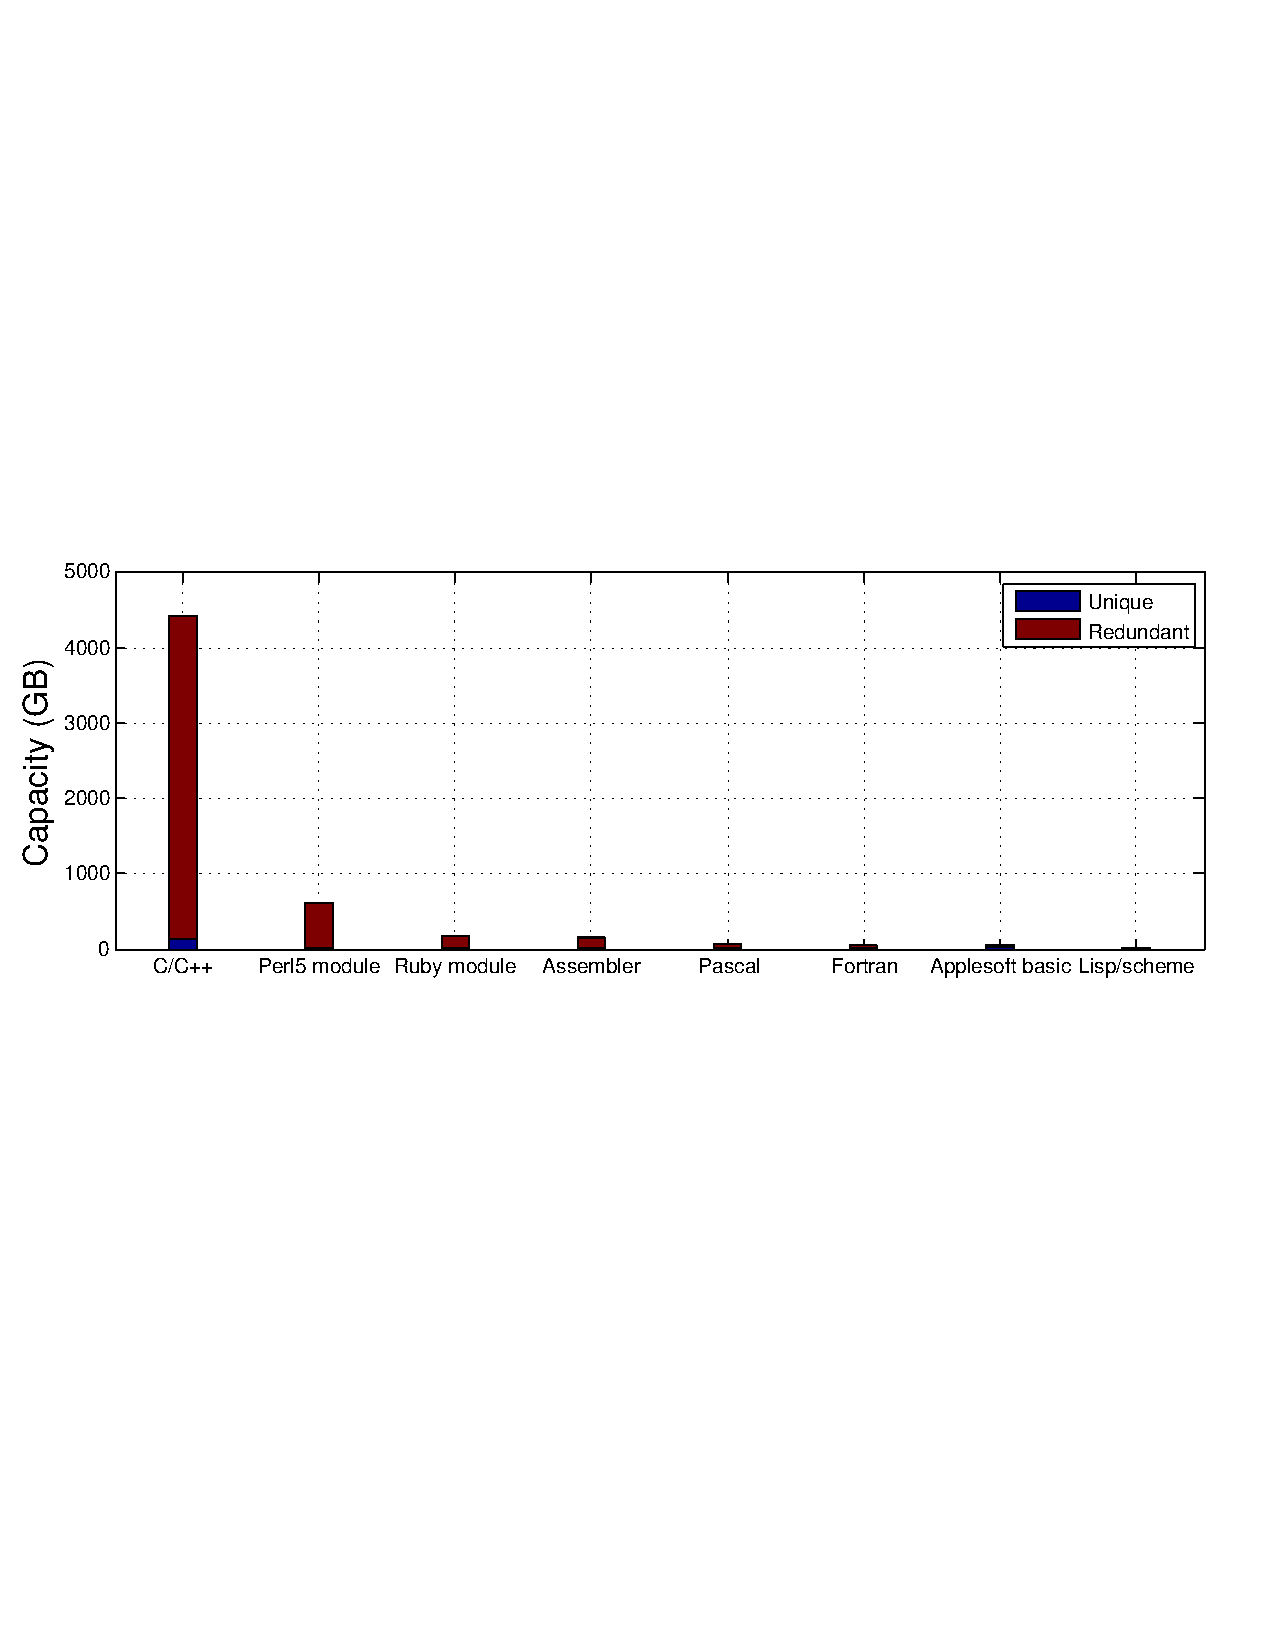
\includegraphics[width=0.5\textwidth]{graphs/type-lang-cap} %
%%\caption{Redundant data vs. unique data for source code files.  %	} %
%%\label{fig:type-source} %\end{figure}
%%
%%%Figure~\ref{fig:type-lib} shows the redundant library distribution. We see
%%that Gcc precompiled header files have the lowest number of redundant library
%%files (20.3\%), but they take up to 0.93 TB. Almost 86.4\% of redundant
%%library files are Palm libraries, which only take up to 7.2GB space,
%%indicating that gcc compiled header files are much bigger than other
%%libraries.  % %We also found there are different libraries used in layers,
%%such as netcdf library, Ocaml lib., mach-o lib.
%%
%%%Figure~\ref{fig-elf} %\subsection{Lib} % %library files contains libtool
%%library file, OCaml native library, MIT scheme, Mach-O library, OCaml library,
%%Palm OS dynamic library data, Microsoft c/c++ library.current ar archive
%%random library, and other library.
%%%%libtool\|OCaml\|Palm\|MIT\|microsoft\|current ar archive random
%%library\|mach-o\|rpm\|gzip %\subsection{Source code}
%%
%\paragraph{Scripts(Scr.)}
%%%Finding 2: 53.6\% (238,353,674) of redundant scripts are Python scripts,
%%which take up over 2.6TB storage space, indicating that users are more prone
%%to replicate Python scripts compare to other scripts.
%%
%%%\begin{figure} %	\centering %
%%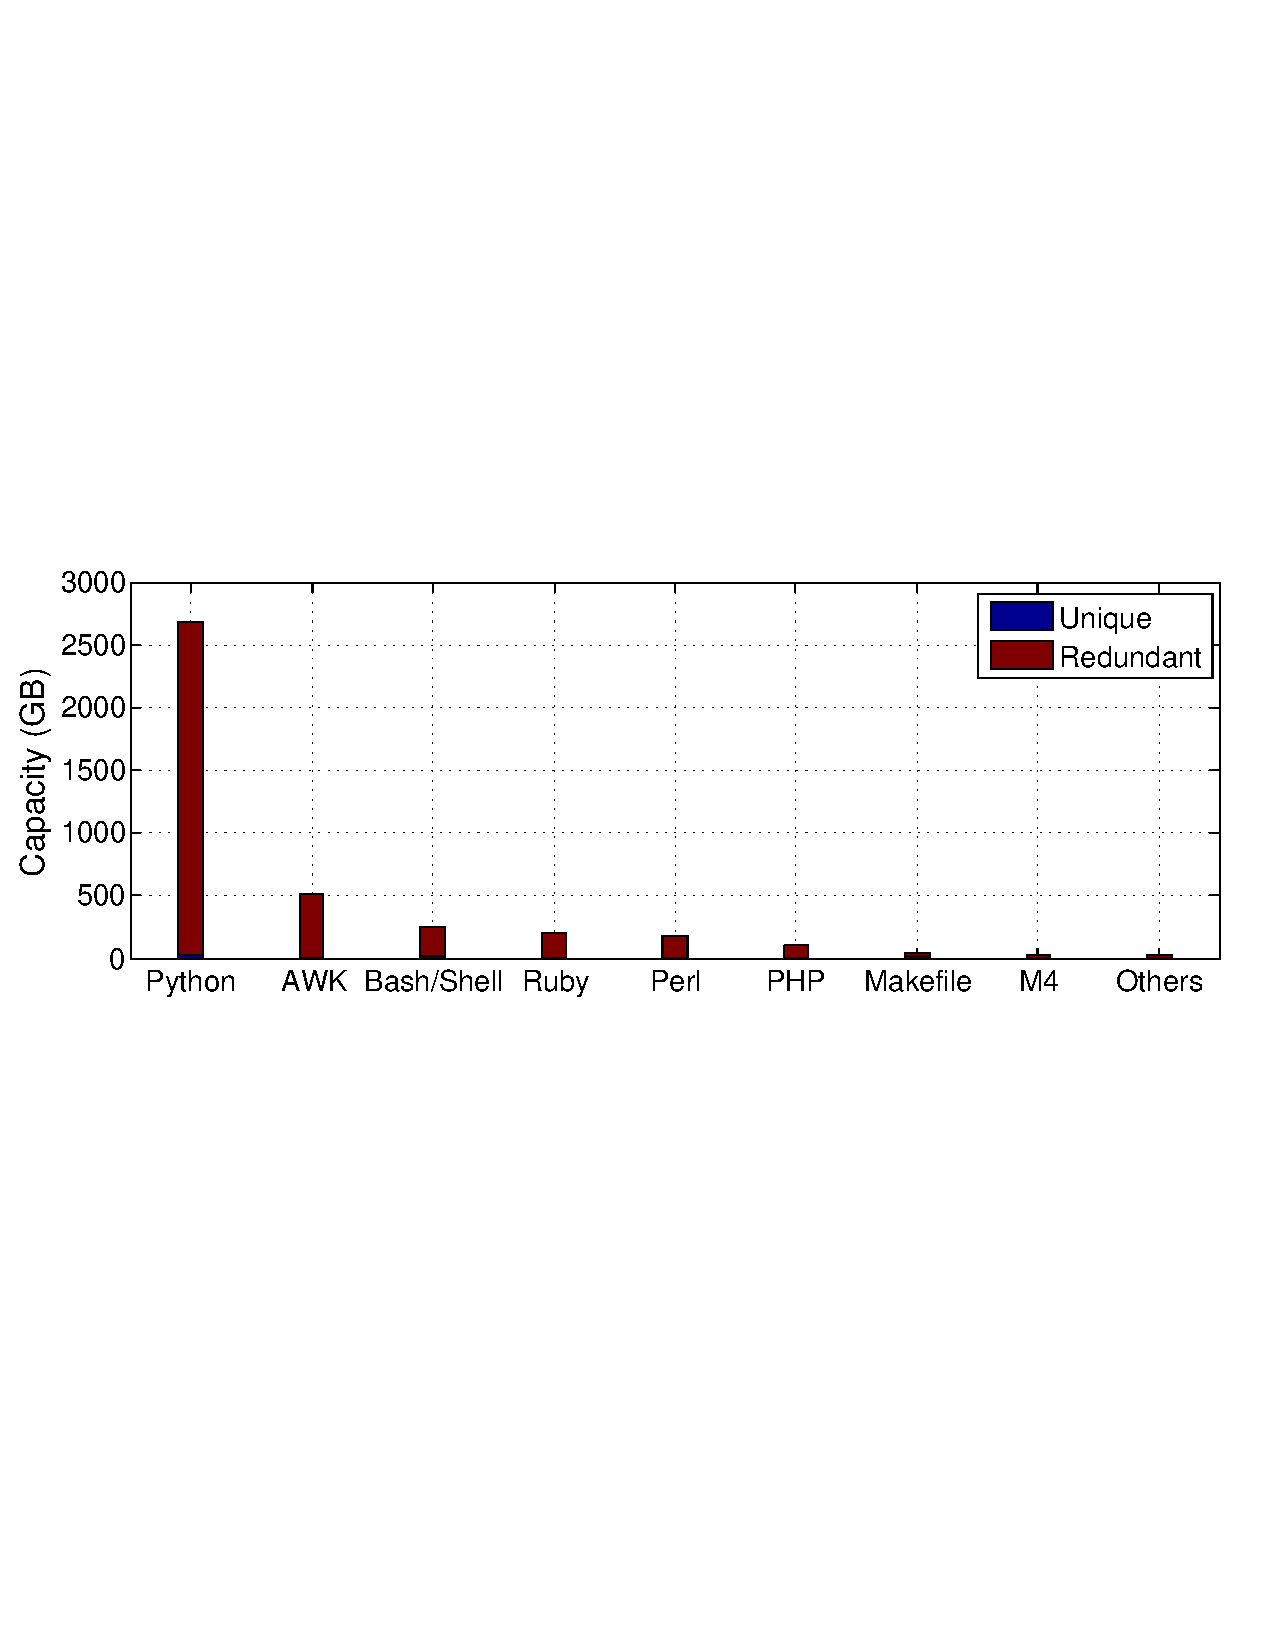
\includegraphics[width=0.5\textwidth]{graphs/type-script-cap} %
%%\caption{Redundant data vs. unique data for scripts.  %	} %
%%\label{fig:type-script} %\end{figure}
%%
%
%\begin{figure} 
%	\centering
%	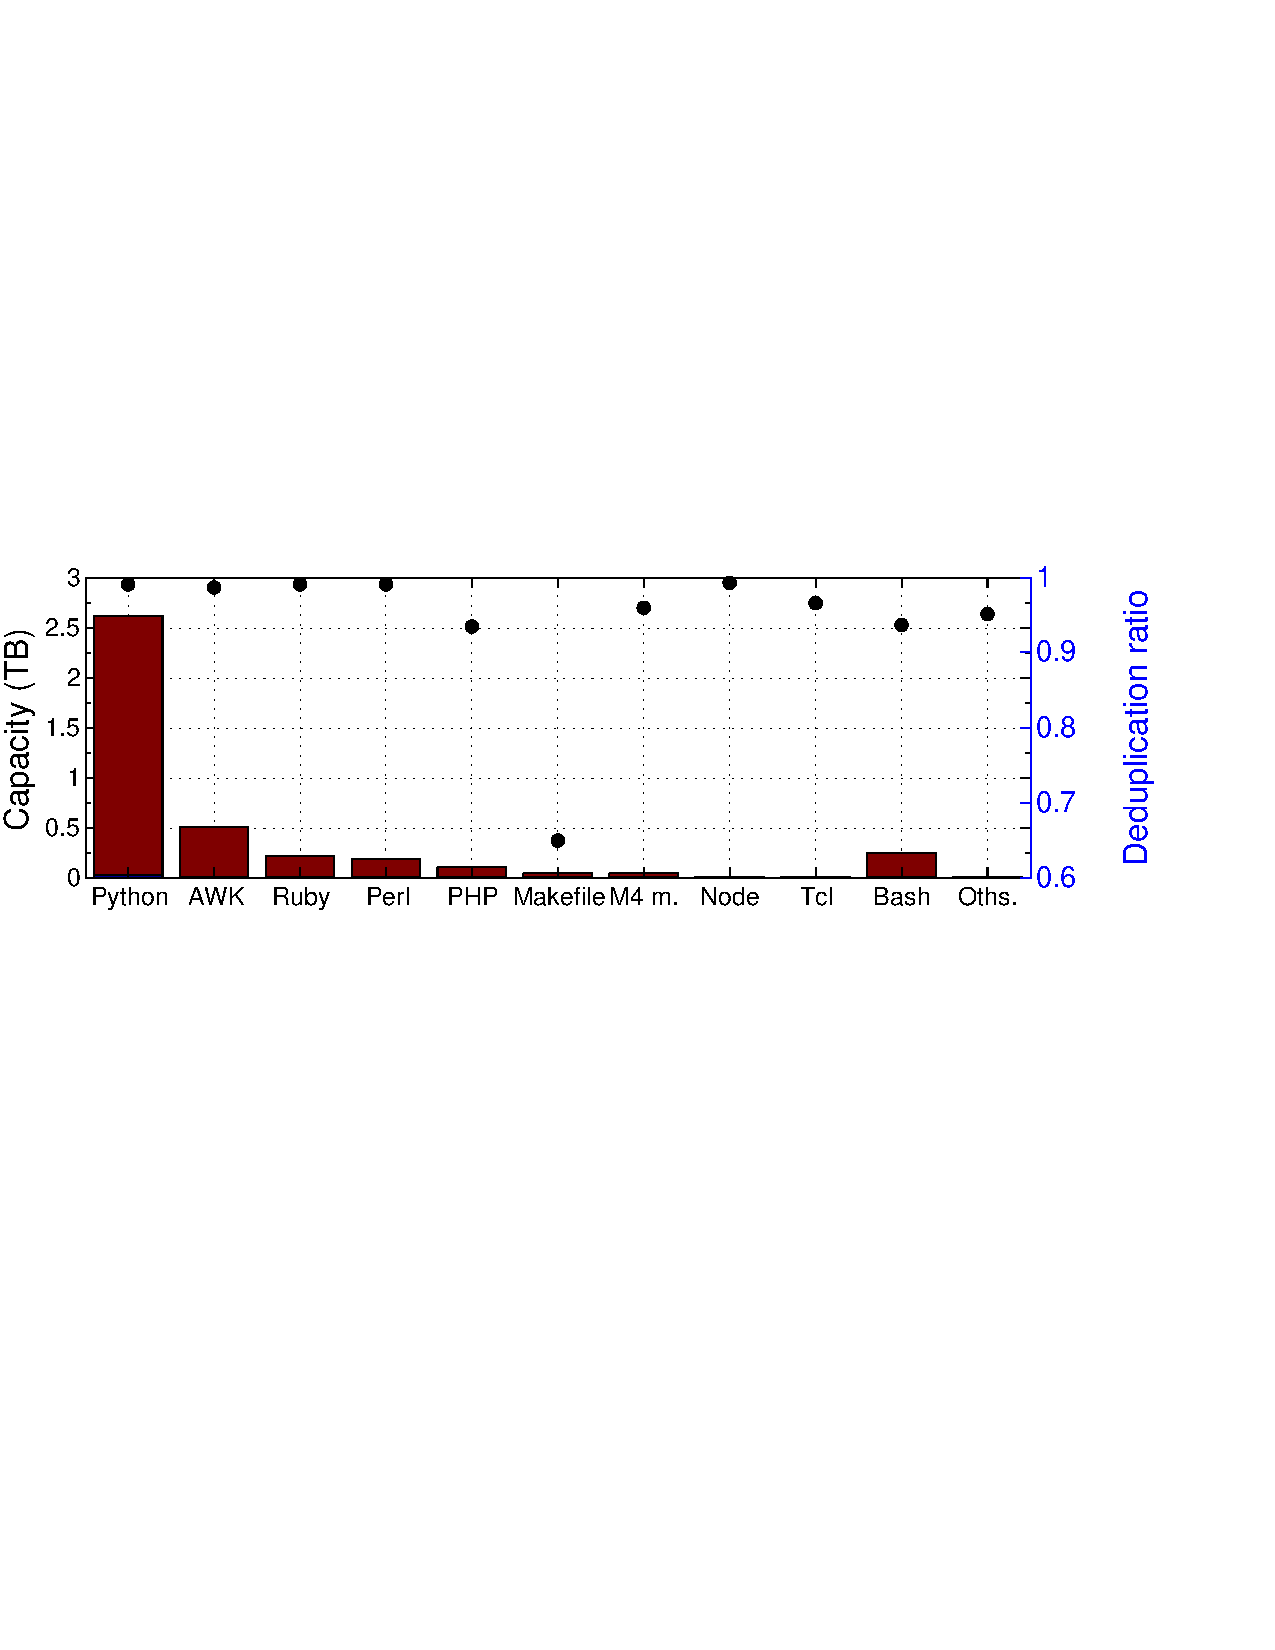
\includegraphics[width=0.45\textwidth]{graphs/dedup-scrp}
%	\caption{Deduplication results for scripts: python, AWK, ruby, perl, PHP, makefile, M4 macro processor, node, Tcl, bash and other scripts.}
%	\label{fig:dedup-scrp} 
%\end{figure}
%
%Similar to source codes, we present the deduplication ratio for scripts as
%shown in Figure~\ref{fig:dedup-scrp}.  
%%
%We see that most of the scripts have a
%high deduplication ratio over 95\%. 
%%
%Especially, the redundant Python scripts
%take up over 65\% of capacity occupied by scripts. 
%
%We inspect the Python scripts and found a frequently replicated Python scripts
%called kraken-tools~\cite{krakentools}, which is a tool for managing system
%requirements for kraken-lib~\cite{krakenlib}. 
%%
%kraken-lib is an orchestration and
%cluster-level management system for Kubernetes~\cite{kubernetes}.
%%% a tool for  for Kubernetes cluster.  %kraken-lib %Kubernetes is an open
%%source platform that automates Linux container operations 
%%
%Although kraken-tools seems like an Docker image repository, it is maintained
%in GitHub rather than Docker registry. 
%%
%Interestingly, kraken-lib does not have
%a official repository in Docker Hub but it has a public repository in QUAY
%registry~\cite{quay}.  
%%
%\textit{Similar to source codes, we suggest to create
%more official images in registry for some popular public scripts %, especially
%containerized applications and convince developers to pull them from registry
%as a read-only layer to reduce redundant scripts in registry.}
%
%\textit{Finding 6: Scripts have a very high deduplication ratio. Especially,
%redundant Python scripts contribute a lot to the overall savings. Many
%redundant scripts are replicated from external public repositories such as
%GitHub.  we suggest to create more official images for these public scripts and
%convince developers to pull them from registry.}
%%% shows the redundant scripts distribution. Python script has the largest
%%number of redundant scripts (238353674, 53.6\%), which take up to 2.6TB
%%storage space, indicating that users are more prone to replicate Python
%%scripts compare to other scripts.  %%This finding also explains that why
%%python byte compiled files takes the largest proportion of intermediate % %We
%%find that users use different scripts in the images.  %For example, 20\%,
%%9.7\% and 4.4\% of scripts are bash/shell scripts, ruby scripts, and awk
%%scripts. Other scripts such as perl script (4.2\%), php script(3.9\%),
%%makefile script(1.3\%), and M4 macro processor script(0.7\%) are also used.
%%
%\paragraph{Documents(Doc.)}
%%%Finding 3: 79.7\%, 5.2\%, and 12.4\% of redundant documents are ASCII text,
%%UTF-8/16 text, and HTML/XML/XHTML, which take up over 11TB, 3.4TB, and 3.9TB
%%redundant storage, indicating that users replicate more ASCII text, UTF-8/16
%%text, and HTML/XML/XHTML compare to other documents.
%%
%\begin{figure} 
%	\centering
%	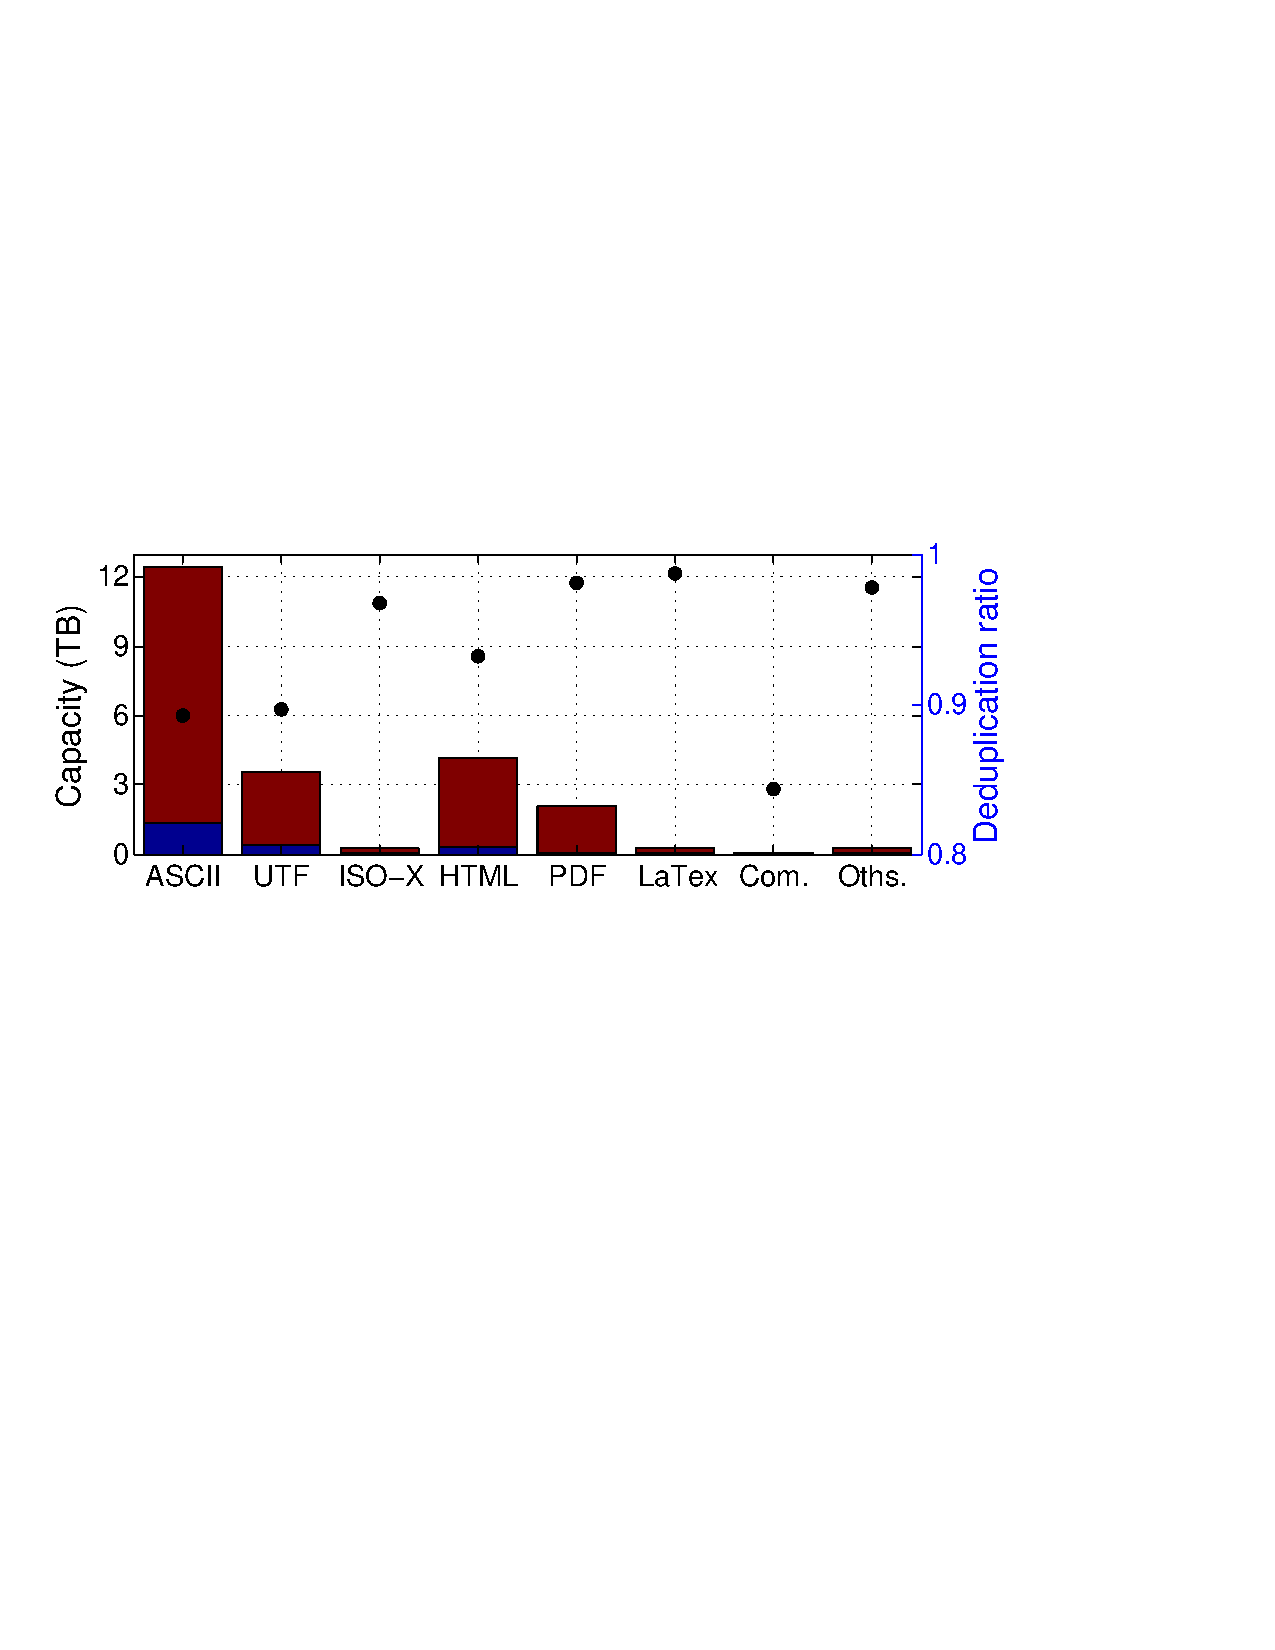
\includegraphics[width=0.35\textwidth]{graphs/dedup-doc} \caption{Deduplication
%	results for documents: ASCII, UTF, ISO-8859, HTML/XML/XHTML, PDF, LaTex
%	documents, Composite document files, and others.} 
%	\label{fig:dedup-doc}
%\end{figure}
%
%Next, we present the deduplication results for different documents as shown in
%Figure~\ref{fig:dedup-doc}.  
%%
%We see that all the documents have a very high
%deduplication ratio of 84\% or higher.  
%%
%Especially, redundant raw text files
%and HTML/XML/XHTML documents take up over 48\% and 17\% of capacity occupied by
%documents. 
%%
%To understand why there are so many document duplicates, we inspect
%raw text files and HTML/XML/XHTML documents respectively. 
%%
%First, we found that
%a large amount of redundant raw text files are input data for testing source
%codes and they are replicated along with source code or script projects from
%external public repositories.  
%%
%For example, scipy~\cite{scipy}, a
%metamathematical software, is replicated from GitHub and stored in different
%images, which contains over 30 raw text files for testing purpose.
%
%Second, after inspected HTML/XML/XHTML documents, we found plenty
%HTML/XML/XHTML documents serves as readme, manual, or license. 
%%
%For example, we
%found plenty redundant HTML documents related to gnome-vfs-doc~\cite{gnome-vfs-doc},
%which are documentation for GNOME virtual filesystem subsystem available
%online~\cite{gvfs}.
%
%\textit{Finding 7: Documents have a very high redundant ratio. Majority
%redundant documents are raw text files and HTML/XML/XHTML documents. They are
%replicated along with source code or script projects and serves as input data
%for testing or informative documents.}
%%
%%%\begin{figure} %	\centering %
%%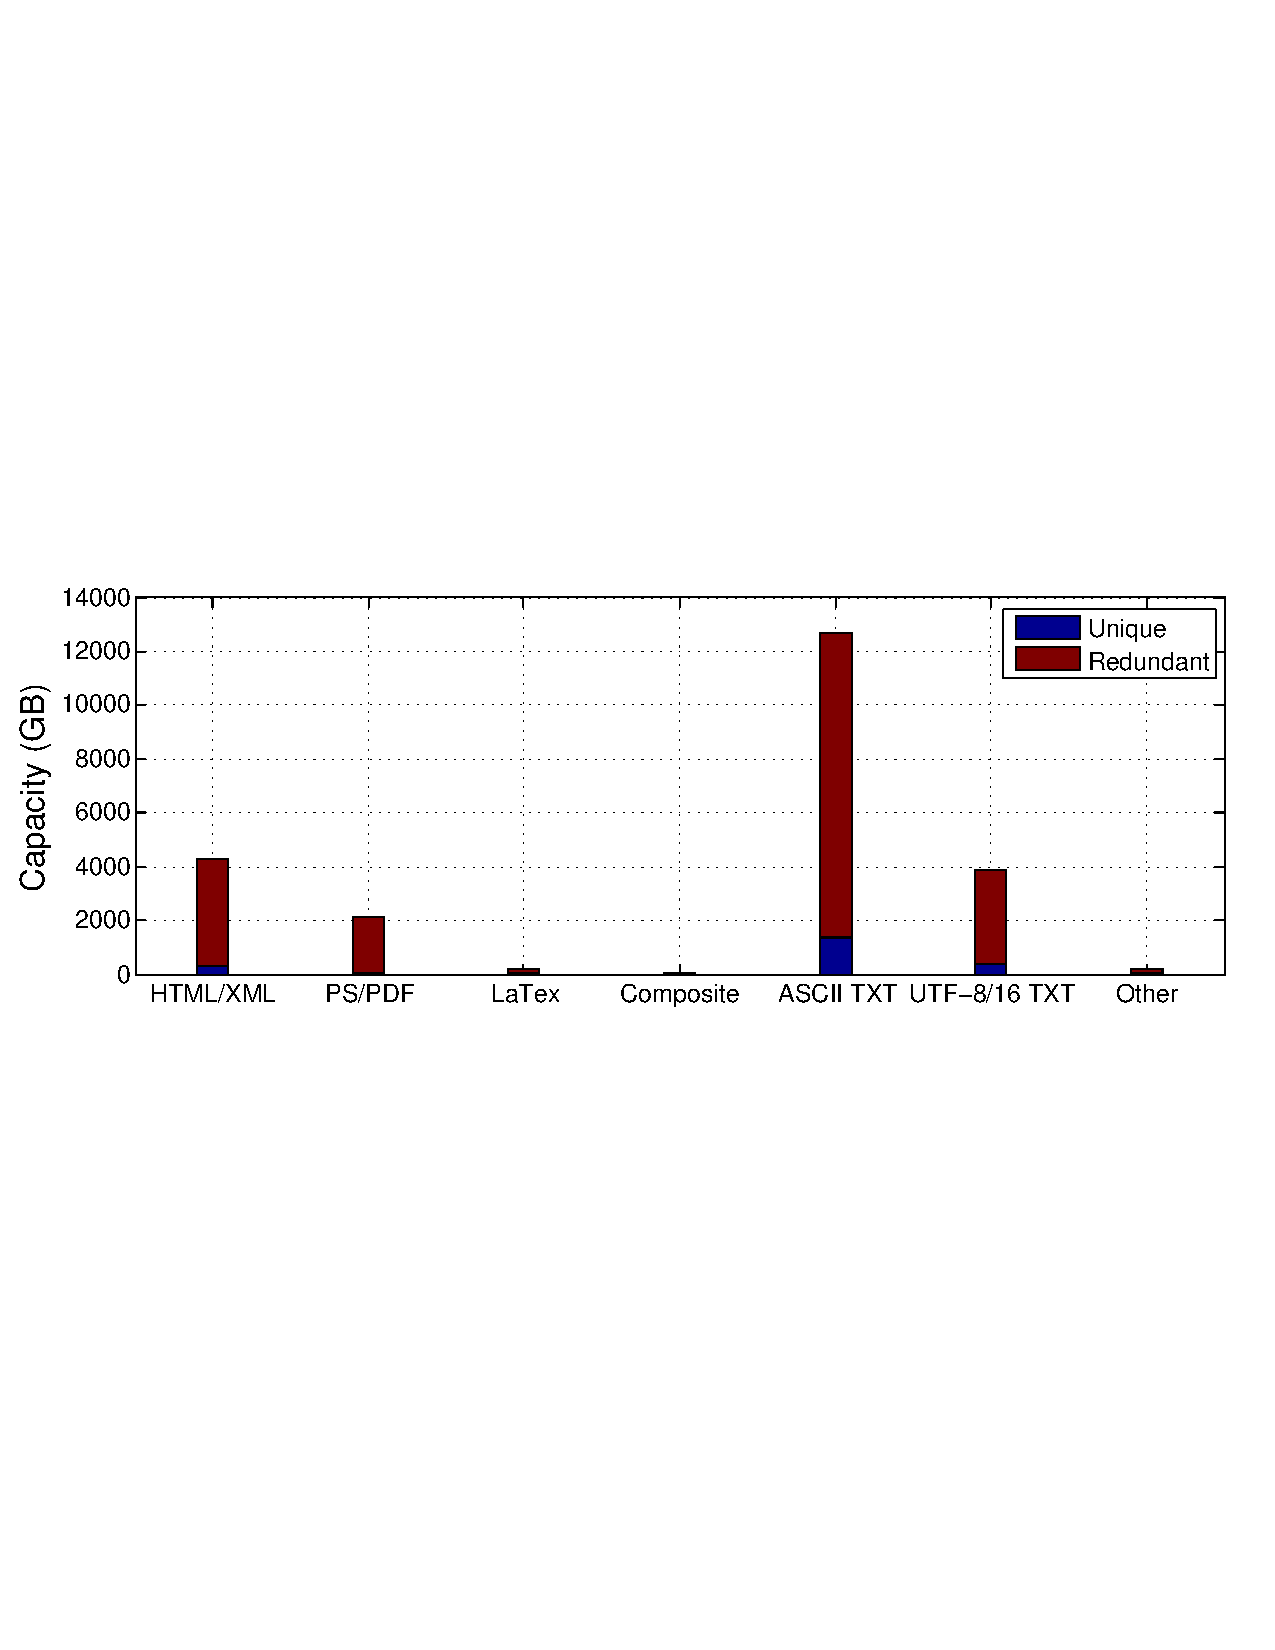
\includegraphics[width=0.5\textwidth]{graphs/type-utili-cap} %
%%\caption{Redundant data vs. unique data for documents.  %	} %
%%\label{fig:type-doc} %\end{figure}
%%
%%%https://pkgs.alpinelinux.org/contents?branch=edge&name=gnome-vfs-doc&arch=x86_64&repo=main
%%% presents redundant document distribution. We first group documents into two
%%categories: non-text documents and raw text documents.  %We see that ASCII
%%text files have the largest number of redundant document files (1,758,299,693,
%%79.7\%), which take up to 11TB storage space, indicating that users replicate
%%more ASCII text.  %12.4\% of the redundant documents are HTML/XML/XHTML
%%documents, which take up to 3.9 TB storage space, indicating users also
%%replicate HTML/XML/XHTML documents in images.  % %In addition to ASCII text,
%%5.2\% of redundant documents are UTF-8/16 unicode text, which take up 3.4 TB
%%storage space.  %Various documents are replicated in images, such as PS/PDF
%%documents (0.9\%), LaTex files (1.1\%) and Composite documents (0.01\%)
%%
%%%79.7\%, 5.2\%, and 12.4\% of redundant documents are ASCII text, UTF-8/16
%%text, and HTML/XML/XHTML, which take up over 11TB, 3.4TB, and 3.9TB redundant
%%storage, indicating that users replicate more ASCII text, UTF-8/16 text, and
%%HTML/XML/XHTML compare to other documents.  %type-utili-cap %type-script-cap
%%
%\paragraph{Databases (DB.)}
%%
%\begin{figure} 
%	\centering
%	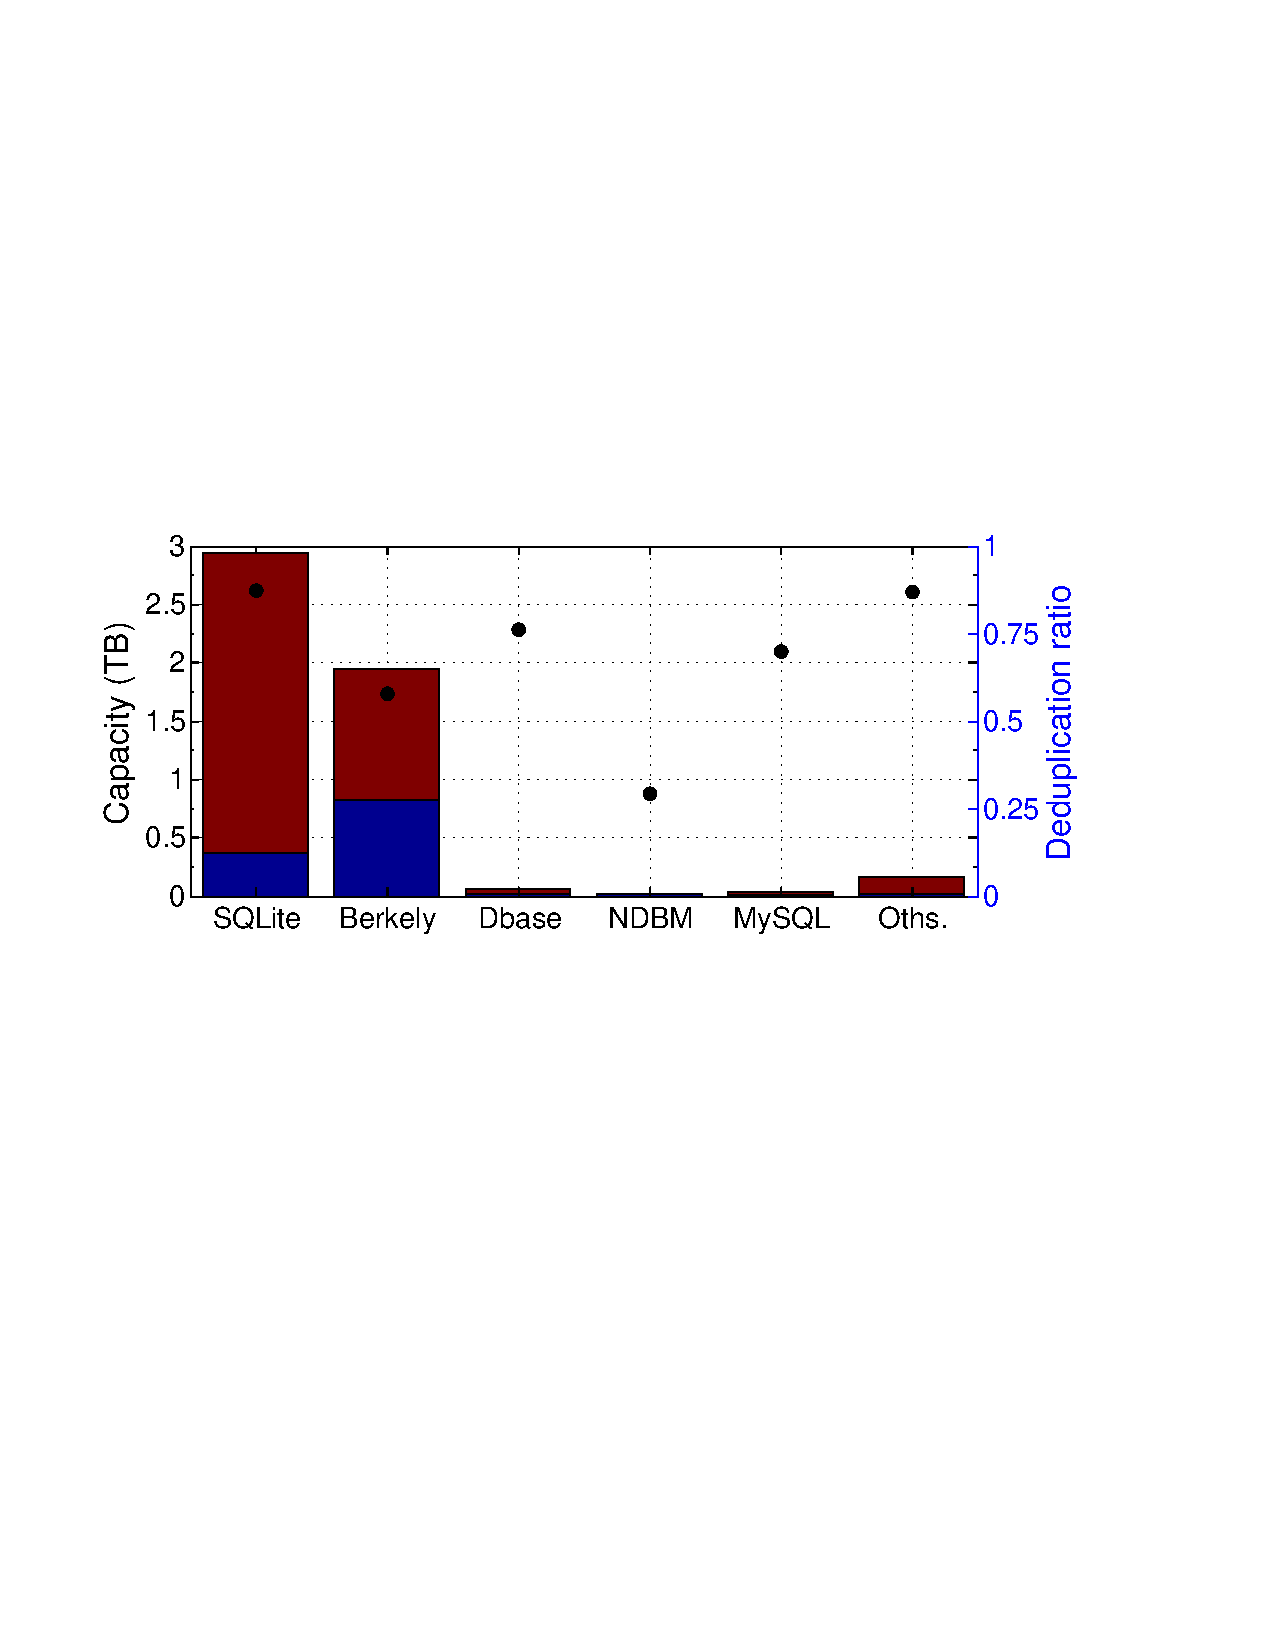
\includegraphics[width=0.4\textwidth]{graphs/dedup-db} \caption{Deduplication
%	results for database related files.  } 
%	\label{fig:dedup-db} 
%\end{figure}
%
%As discussed, Database related files have the lowest deduplication ratio at
%file-level. 
%%
%It makes sense because it's unusual for different users to create
%large amount of identical database files. 
%%
%Figure~\ref{fig:dedup-db} shows the
%deduplication ratio for different types of databases. 
%%
%We see that SQLite
%database files have the largest deduplication ratio of 87\% and could be
%deduplicated for saving up to half of the capacity. 
%%
%To find out why there are
%so many redundant SQLite files, we inspected SQLite files manually and found
%majority of redundant SQLite files are created by Yum~\cite{yum} for
%maintaining a list of well-know repositories.
%
%\textit{Finding 8: Databases have a low deduplication ratio. But SQLite files
%have the largest amount of redundant files and contribute a lot for saving
%capacity. The redundant SQLite files are mainly for saving identical list of
%repositories.}
%%
%%%primary_db.sqlite
%%
%%%Finding 4: 28.7\%, 30.9\%, and 11.9\% of redundant database files are
%%Berkeley DB, Mysql, and Dbase related files, which only take up over 1.1 TB,
%%26 GB, and 47.2 GB redundant storage, indicating that users replicate a lot
%%small database files related to Mysql and Berkeley DB. While there are only
%%7.3\% of SQLite files, which take up over 2.6TB storage space, indicating
%%SQLite files are much bigger than others.  % %Figure~\ref{fig:type-db}
%%presents database related redundant files. 30.9\% of redundant database
%%related files are related to MySQL, which only take up to 26GB storage space
%%while SQLite database related redundant files which only take up 7.3\% of
%%redundant database related files consume 2.56 TB storage space, indicating
%%users replicate more MySQL related files and bigger SQLite database related
%%files. %MySQL related files contains mysql table definitation files, mysql
%%misam index files, and mysql misam compressed data.  %Moreover, we also find
%%different redundant database related files are replicated in Docker images.
%%For example, 28.7\%, 11.86\%, and 5.57\% of redundant database files are
%%Berkeley DB, Dbase, and NDBM related files, which take up over 1.1 TB, 47.2
%%GB, and 7.7 GB redundant storage, indicating that users replicate database
%%files, especially, SQLite and Berkeley DB.  %While there are only 7.3\% of
%%SQLite files, which take up over 2.6TB storage space, indicating SQLite files
%%are much bigger than others.
%%
%%
%%%\begin{figure*}[t] %	\centering %	\begin{minipage}{0.35\textwidth} %
%%\centering %
%%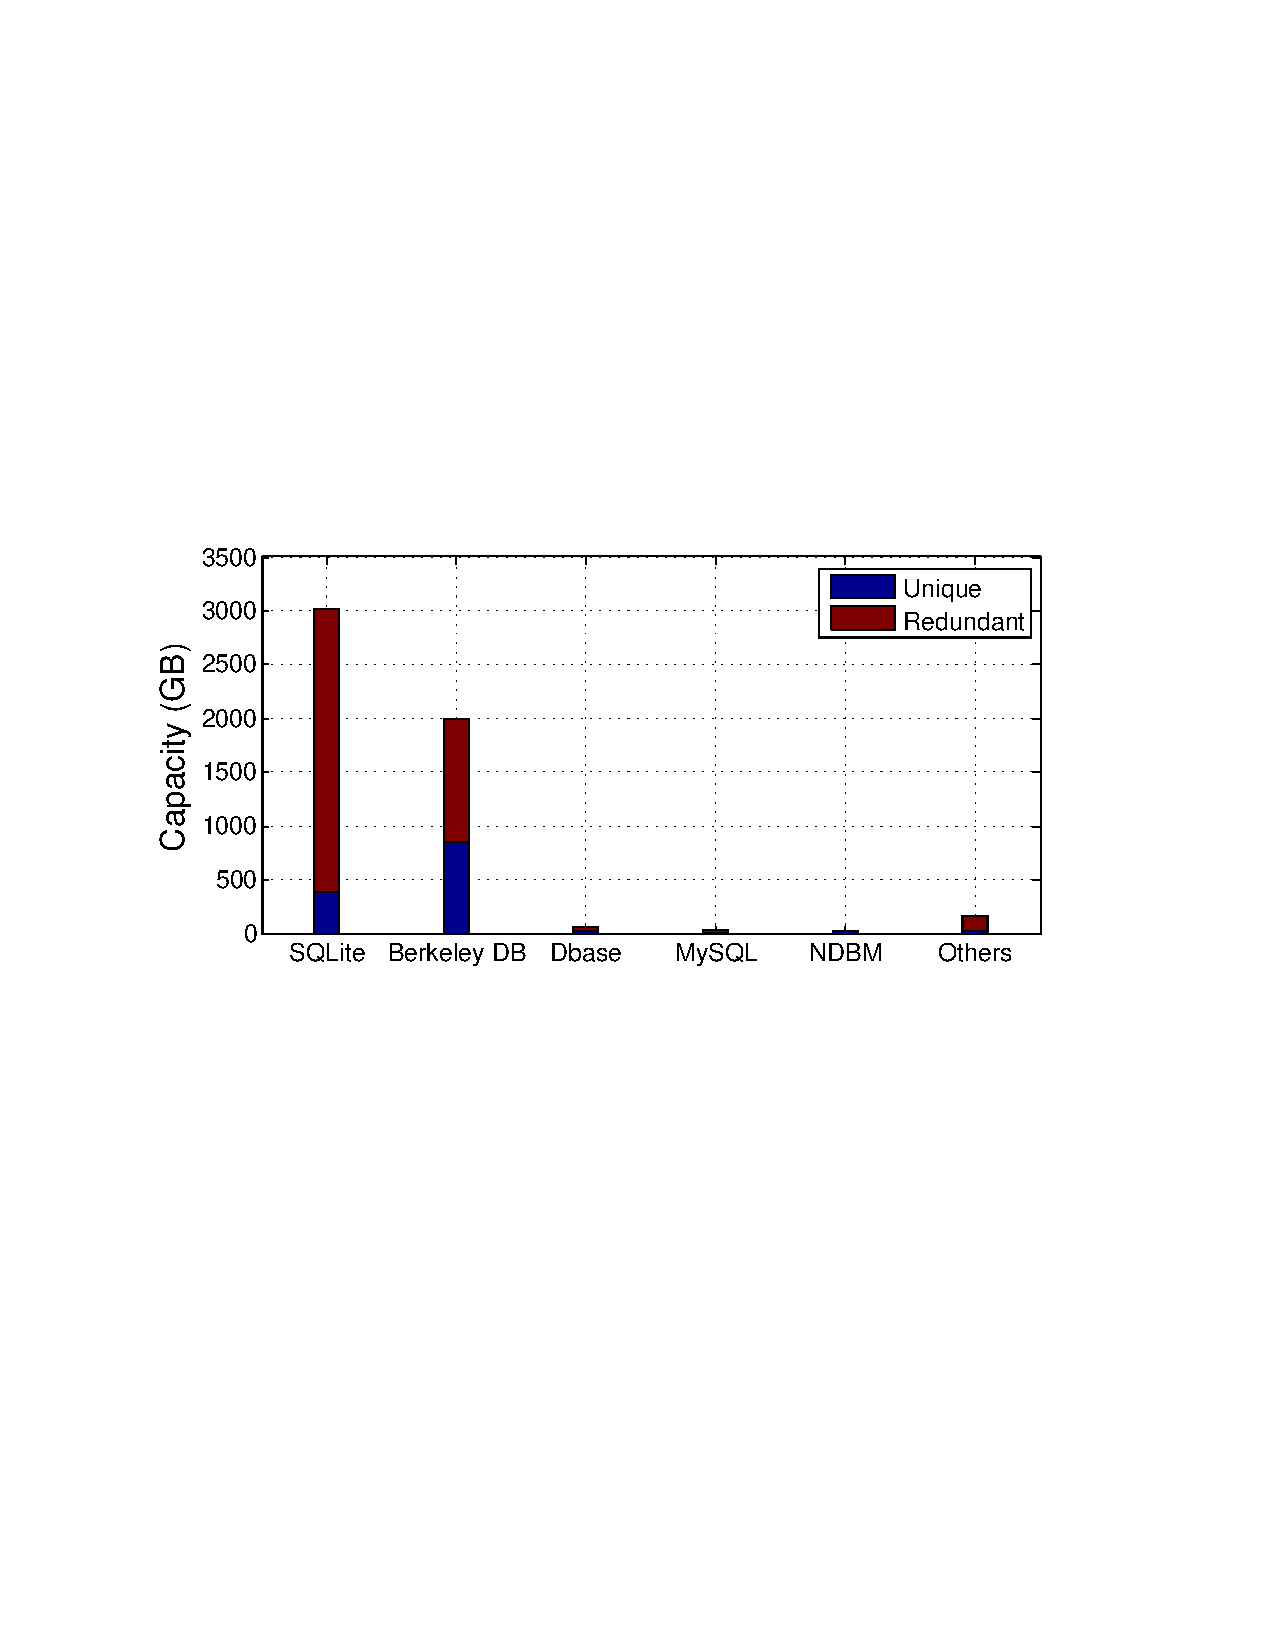
\includegraphics[width=1\textwidth]{graphs/type-db-cap.pdf} %
%%\caption{Redundant data vs. unique data for database related files} %
%%\label{fig:type-db} %	\end{minipage}% %
%%\begin{minipage}{0.278\textwidth} %		\centering %
%%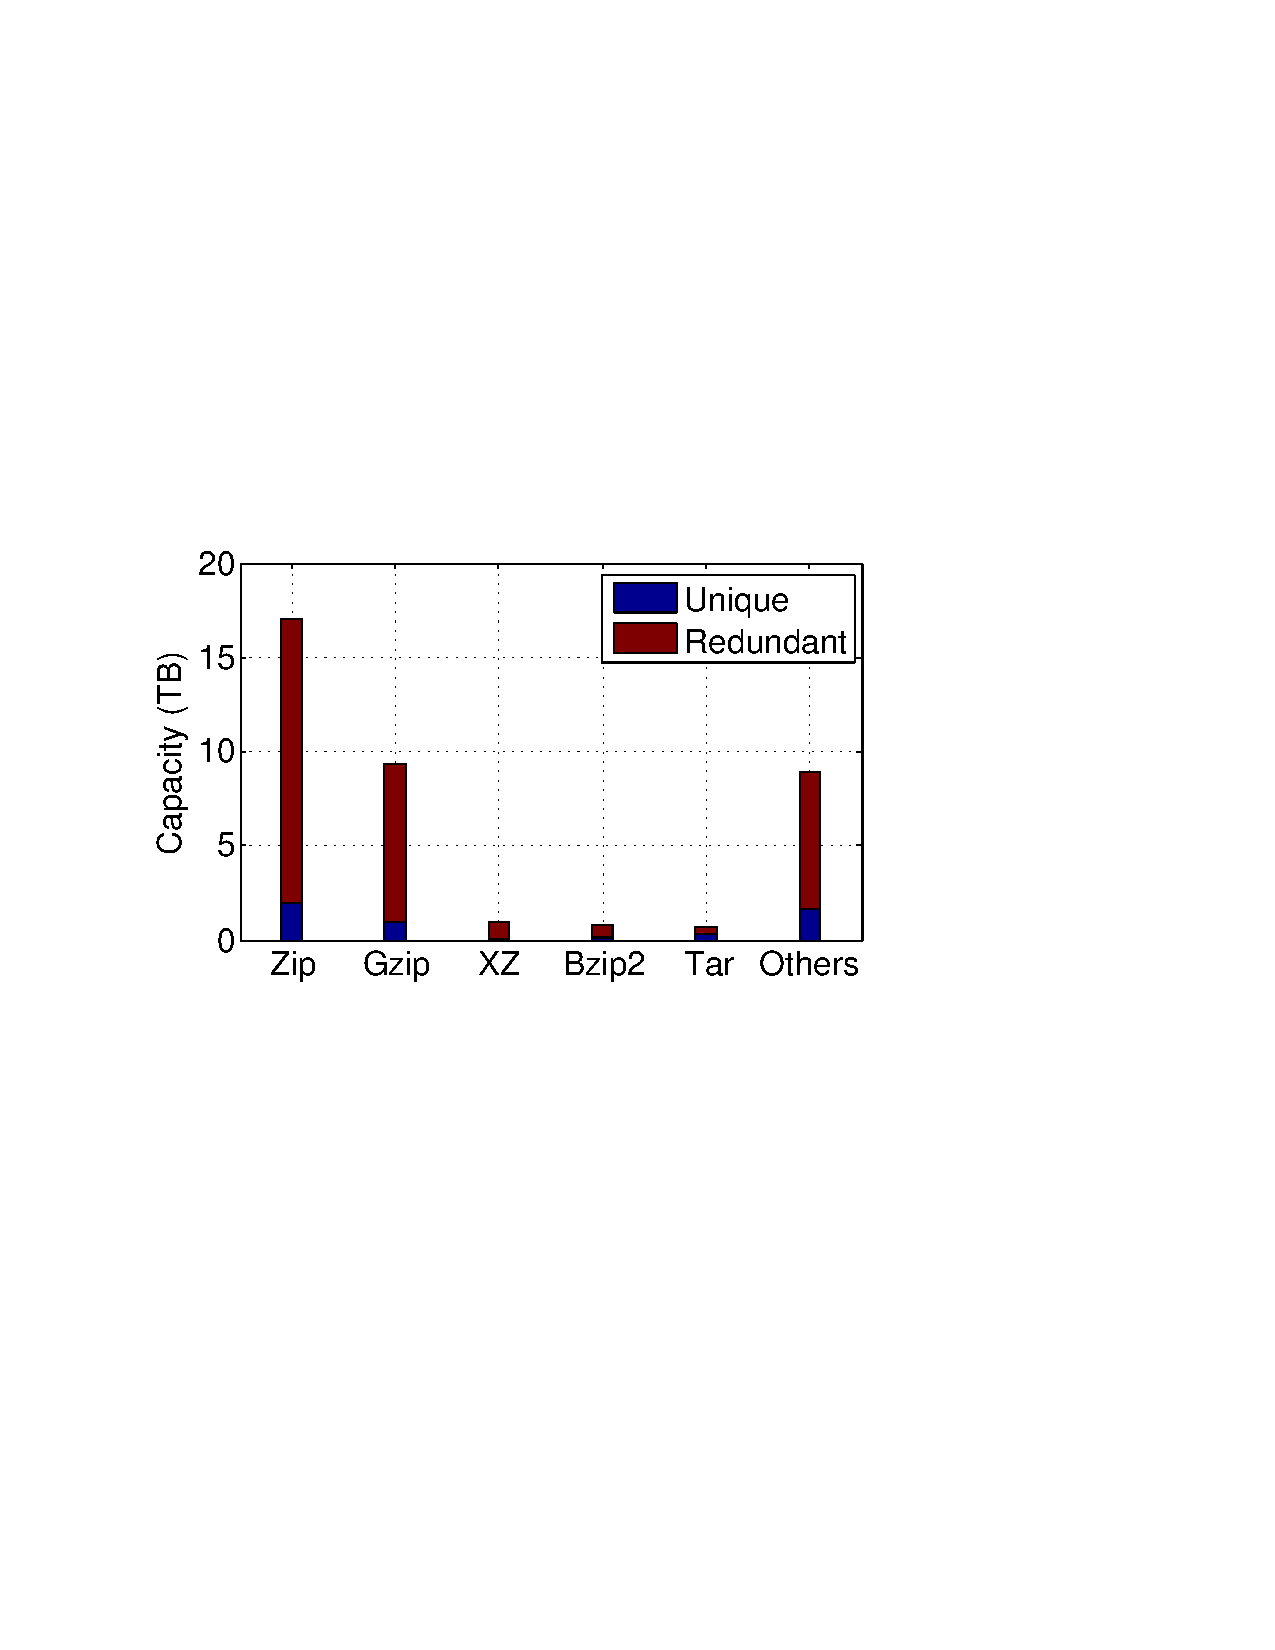
\includegraphics[width=1\textwidth]{graphs/type-tar-type} %
%%\caption{Redundant data vs. unique data for archival files} %
%%\label{fig:type-arch} %	\end{minipage} %
%%\begin{minipage}{0.28\textwidth} %		\centering %
%%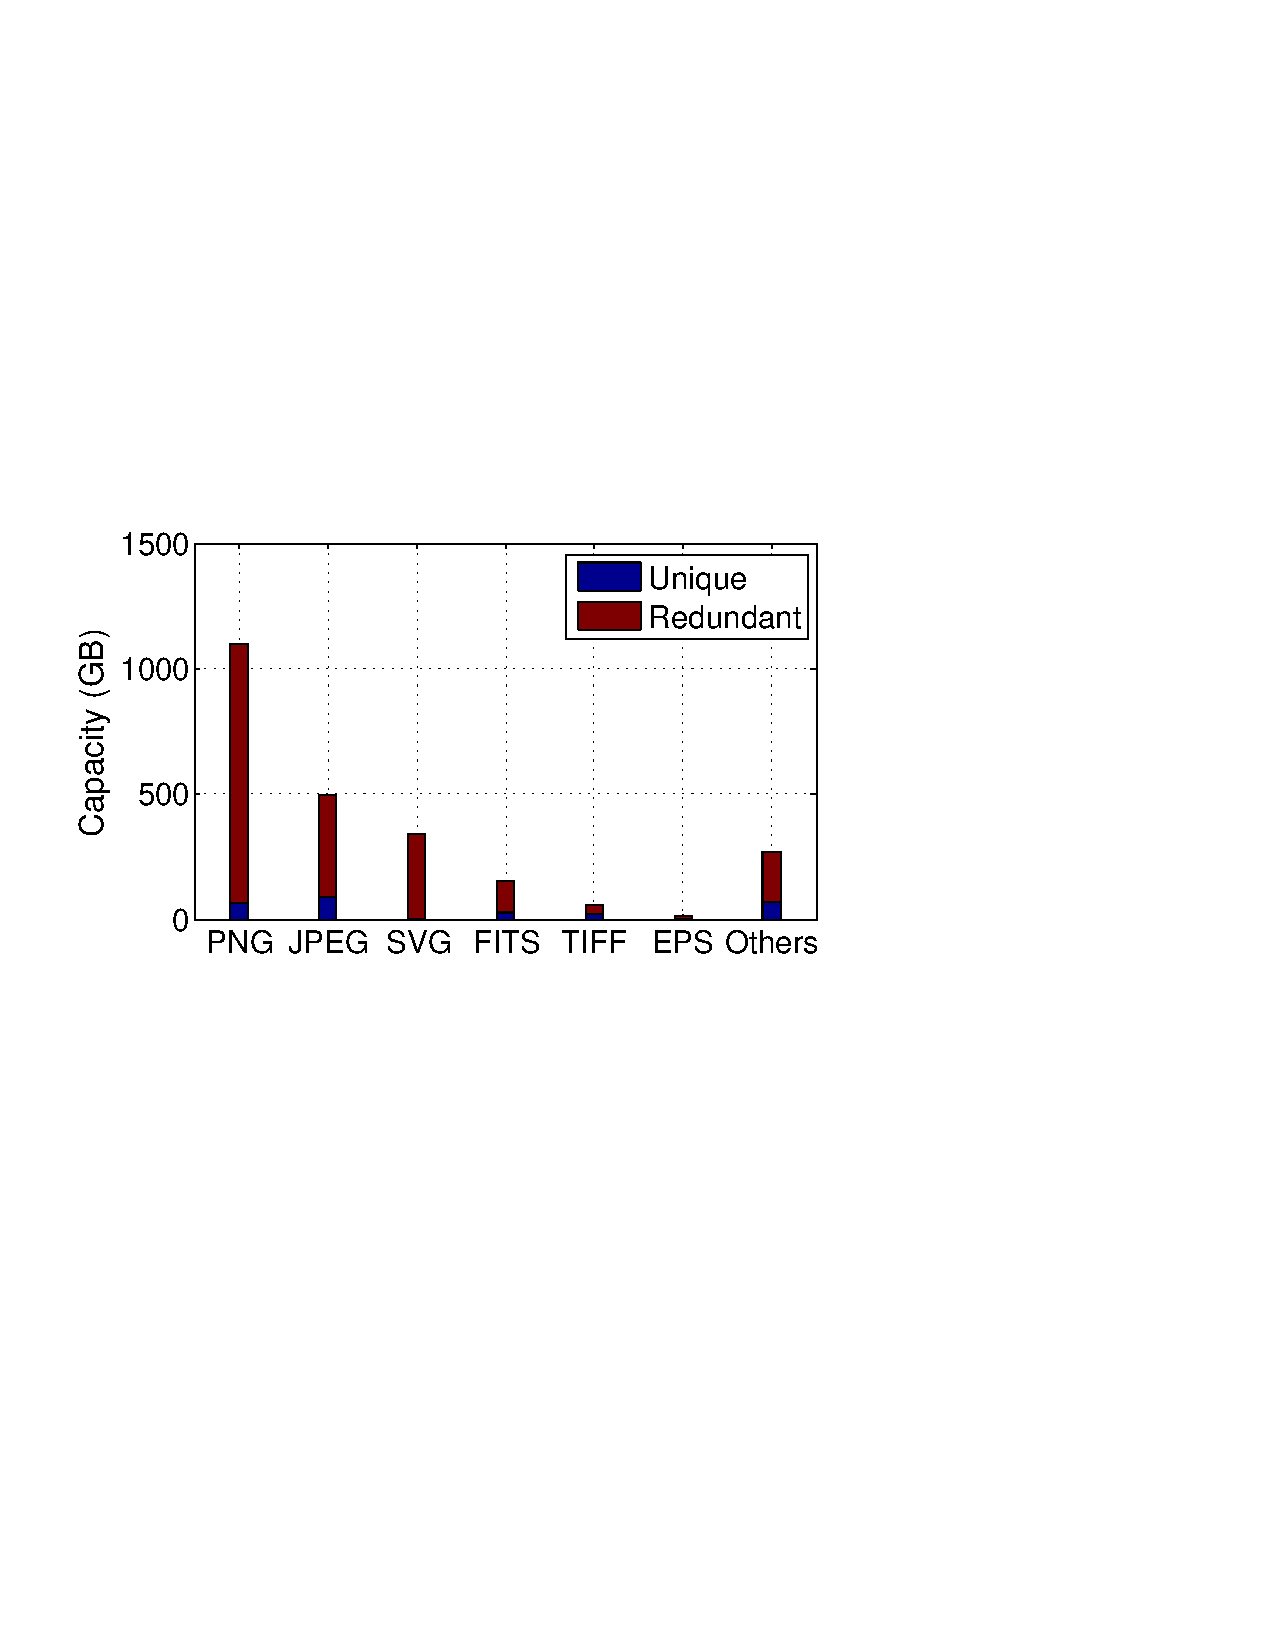
\includegraphics[width=1\textwidth]{graphs/type-image-cap} %
%%\caption{Redundant data vs. unique data for image files} %
%%\label{fig:type-img} %	\end{minipage} %\end{figure*}
%%
%%\paragraph{Archival (Arch.)}
%%
%%Figure~\ref{fig:type-arch} shows the deduplication ratio for each common
%%archival type.  We see that most of archival files have a high deduplication
%%over 80\% except tar archival files. Especially, Zip/Gzip files contribute to
%%most capacity savings after deduplication (62\%).  To understand why there are
%%so many redundant Zip/Gzip files, we manually inspected redundant Zip/Gzip
%%files and found that most of zip/Gzip files packages open source codes.  For
%%example, we found a redundant zip files called android-ndk-r12b.zip. It
%%packages the open source code--Android Native Development Kit (NDK)--that
%%allows Android application developers to include native code in their Android
%%application packages, compiled as JNI shared libraries~\cite{xxx}.
%%android-ndk-r12b.zip is available for downloading from GitHub. 
%%
%%\textit{Finding 9: Archival files have a high deduplication ratio. Majority of
%%Zip/Gzip files packages open source codes that are available online. We
%%suggest developers to remove the redundant archival files after unpacking to
%%reduce image size and save space.}
%%
%%%Finding 4: 89.5\% and 7.0\% of redundant archival files are Gzip files and
%%Zip files, which take up over 8.4 TB and 15.2 TB storage space, indicating
%%that users replicate more Gzip files and Zip files are much bigger than Gzip
%%files.  % % redundant archival file distribution. Gzip files have the largest
%%number of redundant archival files (89.5\%), which take up to 8TB storage
%%space, indicating that users replicate more Gzip compressed files. Although
%%Zip files only take 7.00\% of redundant archival files, they consume 15.5 TB
%%storage space since they are much bigger than Gzip files.  % %We found other
%%different kinds of archive files, such as XZ (0.42\%), Bzip2(0.96\%), and Tar
%%files(0.36\%).
%%
%\paragraph{Images (Img.)}
%
%\begin{figure} \centering
%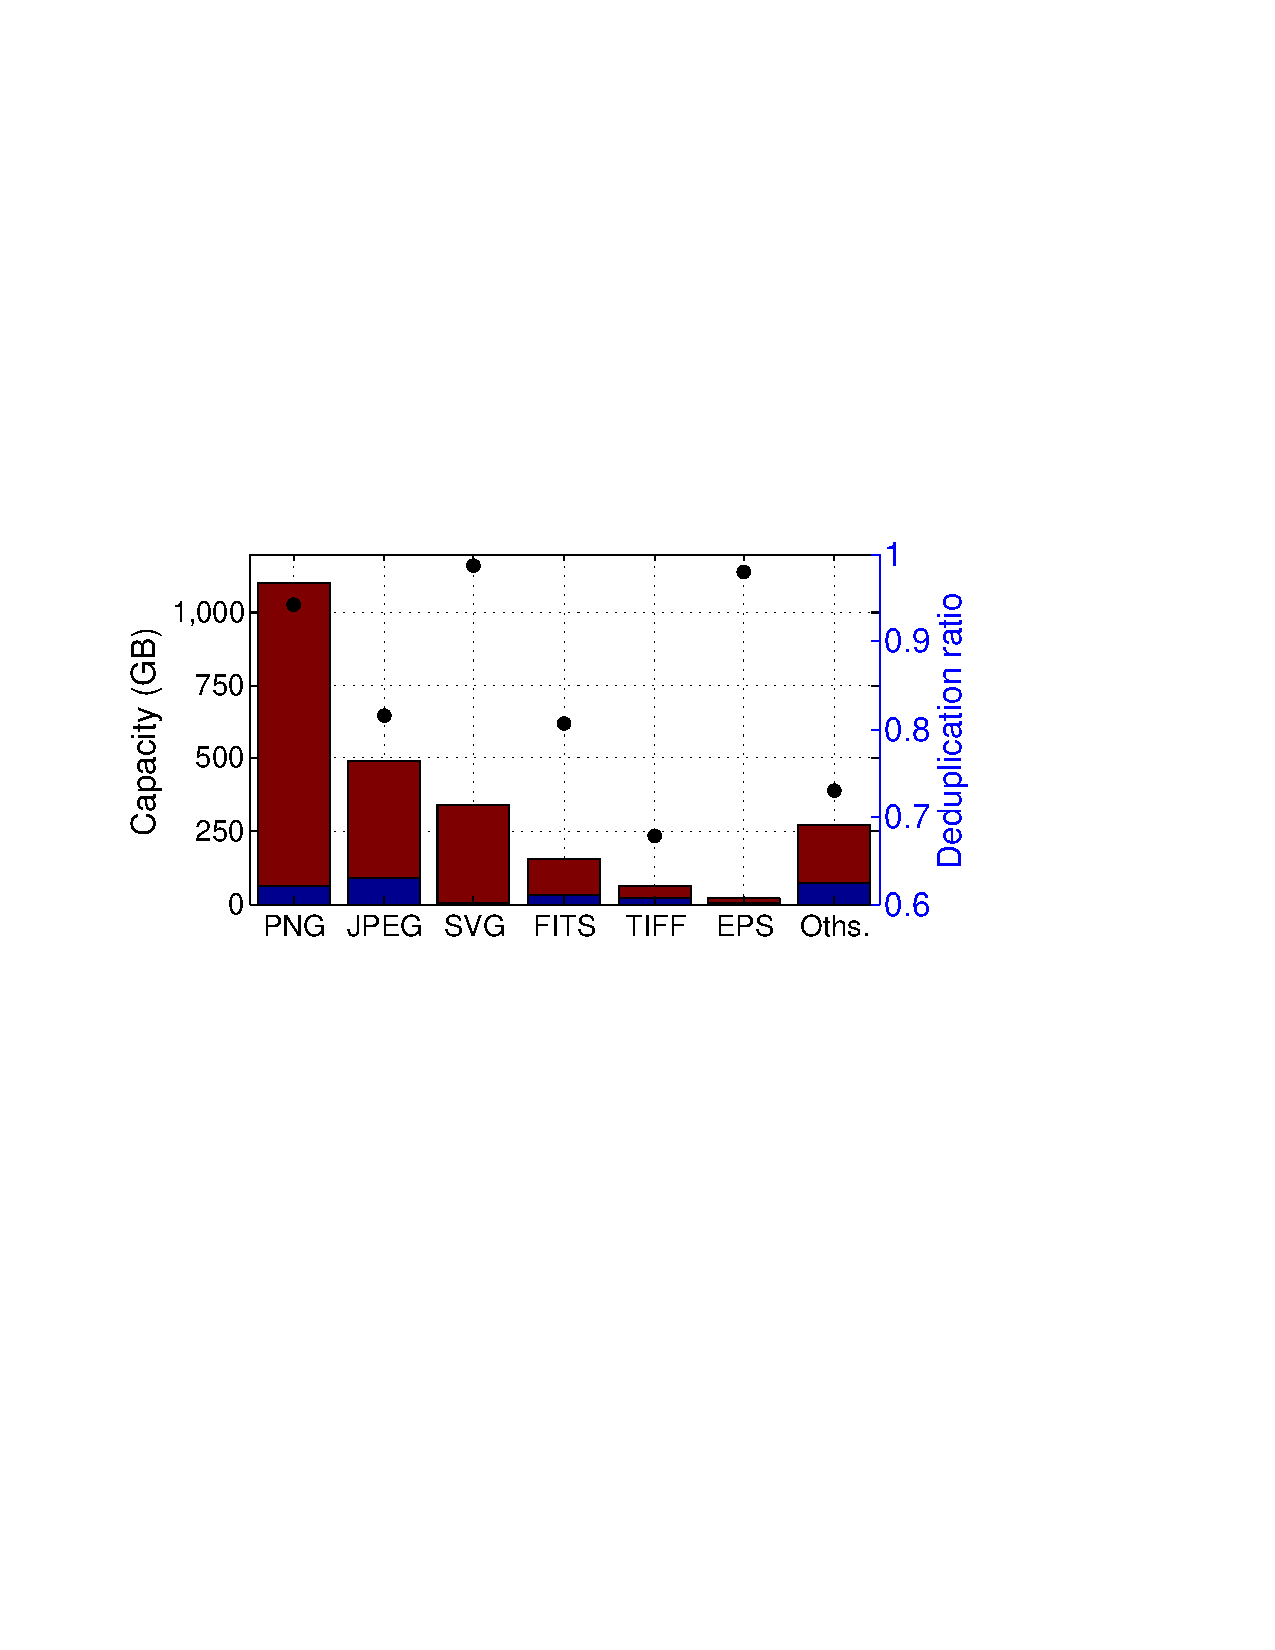
\includegraphics[width=0.35\textwidth]{graphs/dedup-img} \caption{Deduplication
%results for image files.  } \label{fig:dedup-img} \end{figure}
%
%Last, we present the redundant ratio for image files as shown in
%Figure~\ref{fig:dedup-img}.  We see that most of image files have a high
%deduplication ratio over 80\% except TIFF image files and TIFF image files.
%Especially, PNG images contributes to almost half of capacity savings after
%deduplication.  To understand why there are so many redundant image files, we
%inspected redundant PNG images and found plenty of PNG images are logo, icons,
%wallpapers, and images for testing.  For example, we found plenty of redundant
%PNG images related to matplotlib~\cite{matplotlib} for testing purpose. matplotlib is
%a Python 2D plotting library and available on GitHub.
%
%\textit{Finding 10: Most image files have a high deduplication ratio. PNG files
%contribute most to the space savings. Majority redundant PNG files are
%supplementary for documents or testing images for graphic editor softwares.}
%%%Finding 4: 67.8\%, 14.3\%, and 4.0\% of redundant image files are PNG, SVG,
%%and JPEG images, which take up over 1.01TB, 4.6 GB, and 401.5 GB storage
%%space, indicating that users also replicate image files, especially, PNG, SVG,
%%and JPEG files.  % % shows the redundant image file distribution. PNG image
%%files have the largest number of redundant image files (67.8\%), which take up
%%to over 1 TB storage space. 14.3\%, and 4.0\% of redundant image files are
%%SVG, and JPEG images, which take up over 4.6 GB and 401.5 GB storage space,
%%indicating that users also replicate image files, especially, PNG, SVG, and
%%JPEG files. Moreover, there are different redundant image file types, such as
%%FITS (0.05\%), TIFF (0.07\%), and EPS (0.01\%) image files.
%%
%%%\begin{figure} %	\centering %
%%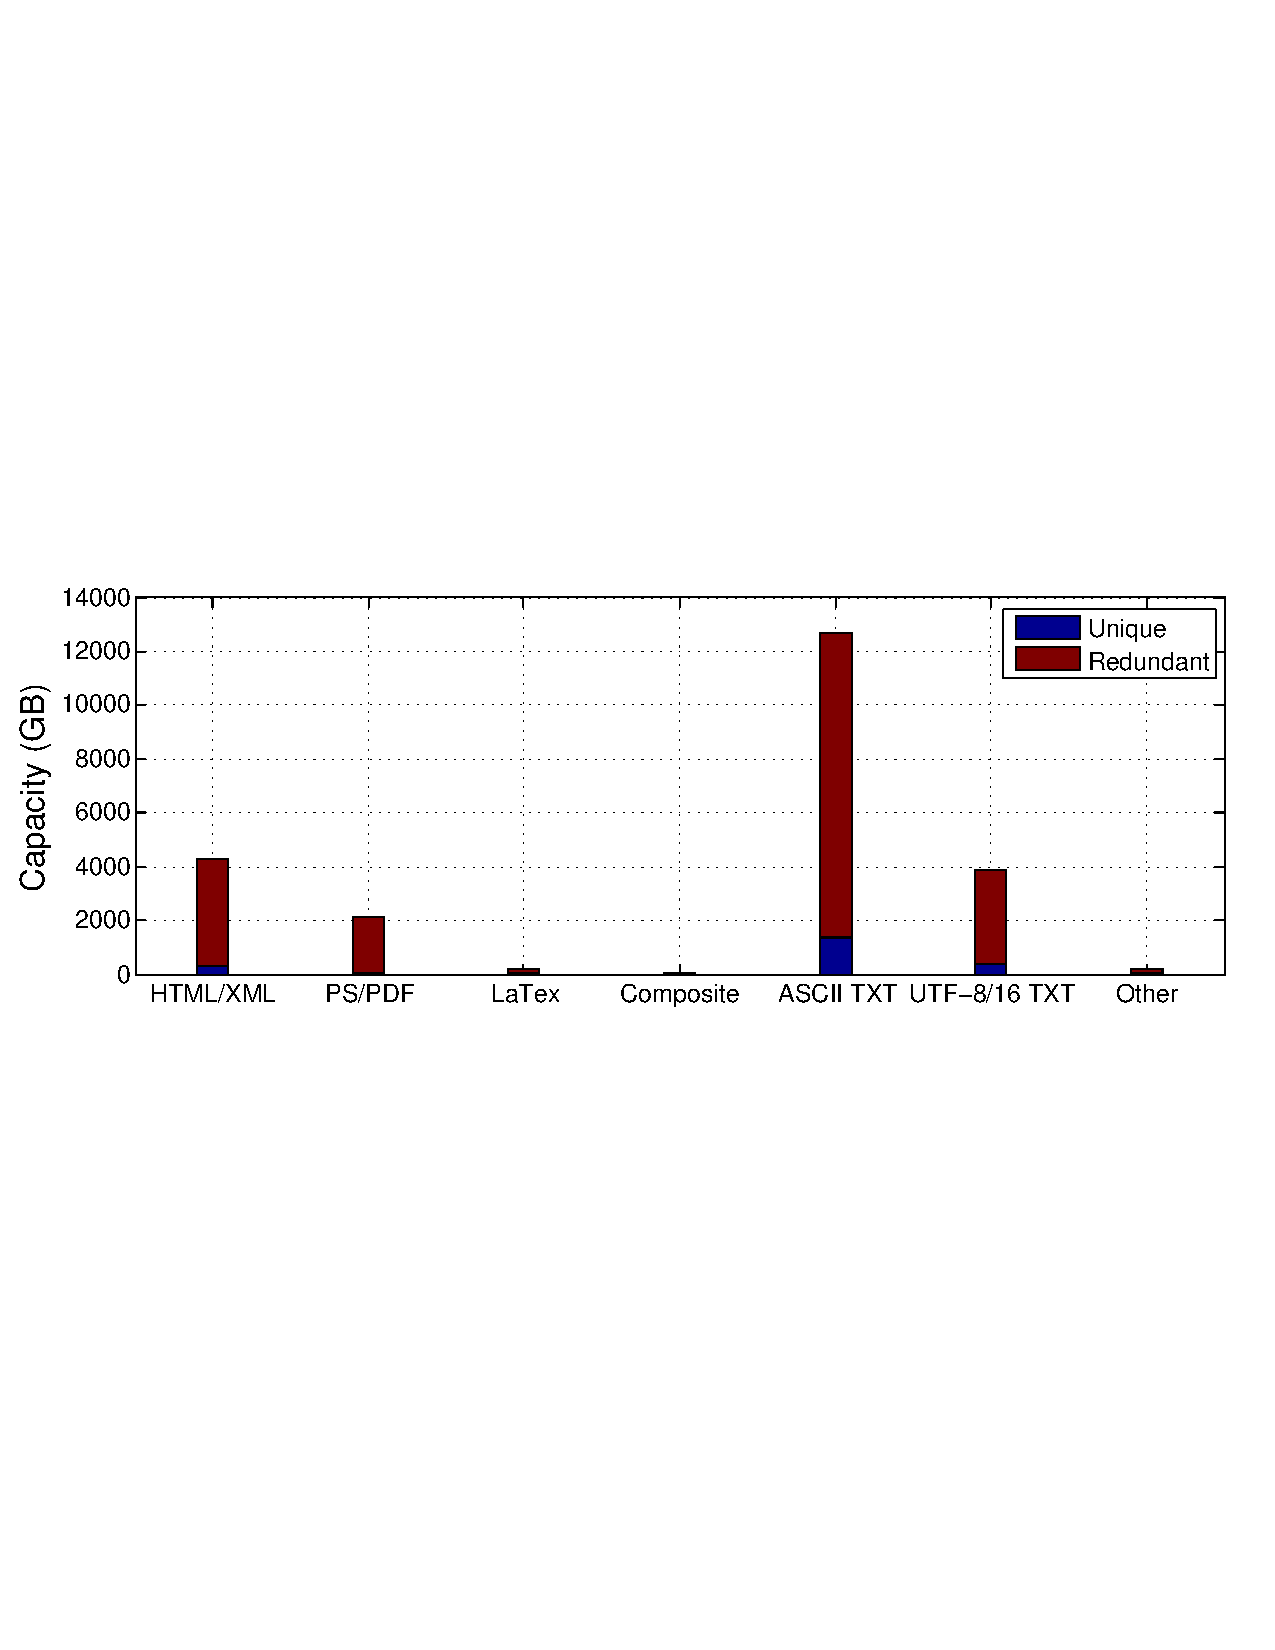
\includegraphics[width=0.35\textwidth]{graphs/type-utili-cap} %
%%\caption{Image file distribution.  %	} %	\label{fig:file_size}
%%%\end{figure}
%%
%%%======================================= %|             OLD VERSION
%%| %=======================================
%%
%%%\begin{table} %	\centering %	\scriptsize  %	\caption{Top 20
%%redundant files' characterization (sorted by repeat cnt.)} %
%%\label{tbl:top_dup_files_repeat_cnt} %
%%\begin{tabular}{|l|l|l|l|l|}%p{0.14\textwidth} %		\hline %
%%Filename & repeat cnt. & type & extension & size \\ %		\hline %
%%&   &   &   &  \\ %		\hline %		&   &   &   &   \\ %
%%\hline %		&   &   &  &    \\ %		\hline %
%%&  &  &  & \\ %		\hline %		& &  &   & \\ %
%%\hline %		& &  &   & \\ %		\hline %		&  &  &
%%& \\ %		\hline %	\end{tabular} %\end{table}
%%
%%%\begin{table} %	\centering %	\scriptsize  %	\caption{Top 20
%%redundant files' characterization (sorted by capacity)} %
%%\label{tbl:top_dup_files_cap} %
%%\begin{tabular}{|l|l|l|l|l|}%p{0.14\textwidth} %		\hline %
%%Filename & repeat cnt. & type & extension & size \\ %		\hline %
%%&   &   &   &  \\ %		\hline %		&   &   &   &   \\ %
%%\hline %		&   &   &  &    \\ %		\hline %
%%&  &  &  & \\ %		\hline %		& &  &   & \\ %
%%\hline %		& &  &   & \\ %		\hline %		&  &  &
%%& \\ %		\hline %	\end{tabular} %\end{table}
%%
%%
%%%\begin{table} %	\centering %	\scriptsize  %	\caption{Top redundant
%%file types} %	\label{tbl:top_dup_types} %
%%\begin{tabular}{|l|l|l|l|l|l|}%p{0.14\textwidth} %		\hline %
%%Type & extension & Num. & size & red. ratio (cnt.)  & red. ratio (cap.)\\ %
%%\hline %		&   &   &  & &   \\ %		\hline %
%%&   &   &  & &    \\ %		\hline %		&   &   &   & &   \\ %
%%\hline %		&  &  &  & & \\ %		\hline %
%%& &  &  & & \\ %		\hline %		& &  & & &  \\ %
%%\hline %		&  &  & & &  \\ %		\hline %
%%\end{tabular} %\end{table} 
%%
%%%\subsection{Redundant ratio for directories} % %\begin{table} %
%%\centering %	\scriptsize  %	%\begin{minipage}{.5\linewidth} %
%%\caption{Inter-dir redundant ratio for dirs in terms of file count and
%%capacity} \label{tbl:intra_dup_ratio_dirs} %
%%\begin{tabular}{|l|l|l|}%p{0.14\textwidth} %		\hline %
%%% after \\: \hline or \cline{col1-col2} \cline{col3-col4} ...  %
%%% after \\: \hline or \cline{col1-col2} \cline{col3-col4} ...  %
%%& File count & Capacity \\ %		\hline %		Avg. & 98.75\%
%%& 97.33\%\\ %		\hline %		Median & - & - \\ %
%%\hline %		Max. & 1 & 1\\ %		\hline %
%%Min.  & 0.87\%  & $<$ 0.00\%\\ %		\hline %		Stdev.
%%&  4.70\% & 10.49\\ %		\hline %		Layer dataset after
%%share.-dedup (Uncompressed) & -  & -\\ %		\hline %
%%Total layer dataset (Uncompressed) &  -	& -\\ %		\hline %
%%\end{tabular} %\end{table} % %\begin{table} %	\centering %	\scriptsize  %
%%%\begin{minipage}{.5\linewidth} %	\caption{Intra-dir redundant ratio for
%%dirs in terms of file count and capacity} \label{tbl:inter_dup_ratio_dirs} %
%%\begin{tabular}{|l|l|l|}%p{0.14\textwidth} %		\hline %
%%% after \\: \hline or \cline{col1-col2} \cline{col3-col4} ...  %
%%% after \\: \hline or \cline{col1-col2} \cline{col3-col4} ...  %
%%& File count & Capacity \\ %		\hline %		Avg. & 98.75\%
%%& 97.33\%\\ %		\hline %		Median & - & - \\ %
%%\hline %		Max. & 1 & 1\\ %		\hline %
%%Min.  & 0.87\%  & $<$ 0.00\%\\ %		\hline %		Stdev.
%%&  4.70\% & 10.49\\ %		\hline %		Layer dataset after
%%share.-dedup (Uncompressed) & -  & -\\ %		\hline %
%%Total layer dataset (Uncompressed) &  -	& -\\ %		\hline %
%%\end{tabular} %\end{table}
%%
%%%\subsection{Redundant directory characterization} % %\begin{table} %
%%\centering %	\scriptsize  %	%\begin{minipage}{.5\linewidth} %
%%\caption{Top redundant dirs'characterization} %
%%\label{tbl:top_dup_dirs} %	\begin{tabular}{|l|l|l|l|}%p{0.14\textwidth} %
%%\hline %		% after \\: \hline or \cline{col1-col2}
%%\cline{col3-col4} ...  %		% after \\: \hline or \cline{col1-col2}
%%\cline{col3-col4} ...  %		Name & Num. & Redundant ratio & Avg.
%%size \\ %		\hline %		home &   &   &     \\ %
%%\hline %		&   &   &      \\ %		\hline %
%%&   &   &      \\ %		\hline %		&  &  &  \\ %
%%\hline %		& &  &   \\ %		\hline %		& &  &
%%\\ %		\hline %		&  &  & \\ %		\hline %
%%\end{tabular} %\end{table} 
%%
%%%\begin{figure} %	\centering %
%%\includegraphics[width=0.5\textwidth]{graphs/} %	\caption{CDF of file
%%repeat count.  %	} %	\label{fig:file_repeat_count} %\end{figure}
%%
%%%\paragraph{Cumulative distribution and probability distribution of file size
%%in terms of unique file size, redundant file size, overall file size}
%%
%%
%%%\paragraph{Average file size by repeat count} % %There is no relation between
%%file repeat count and average file size.  % %\begin{figure} %	\centering %
%%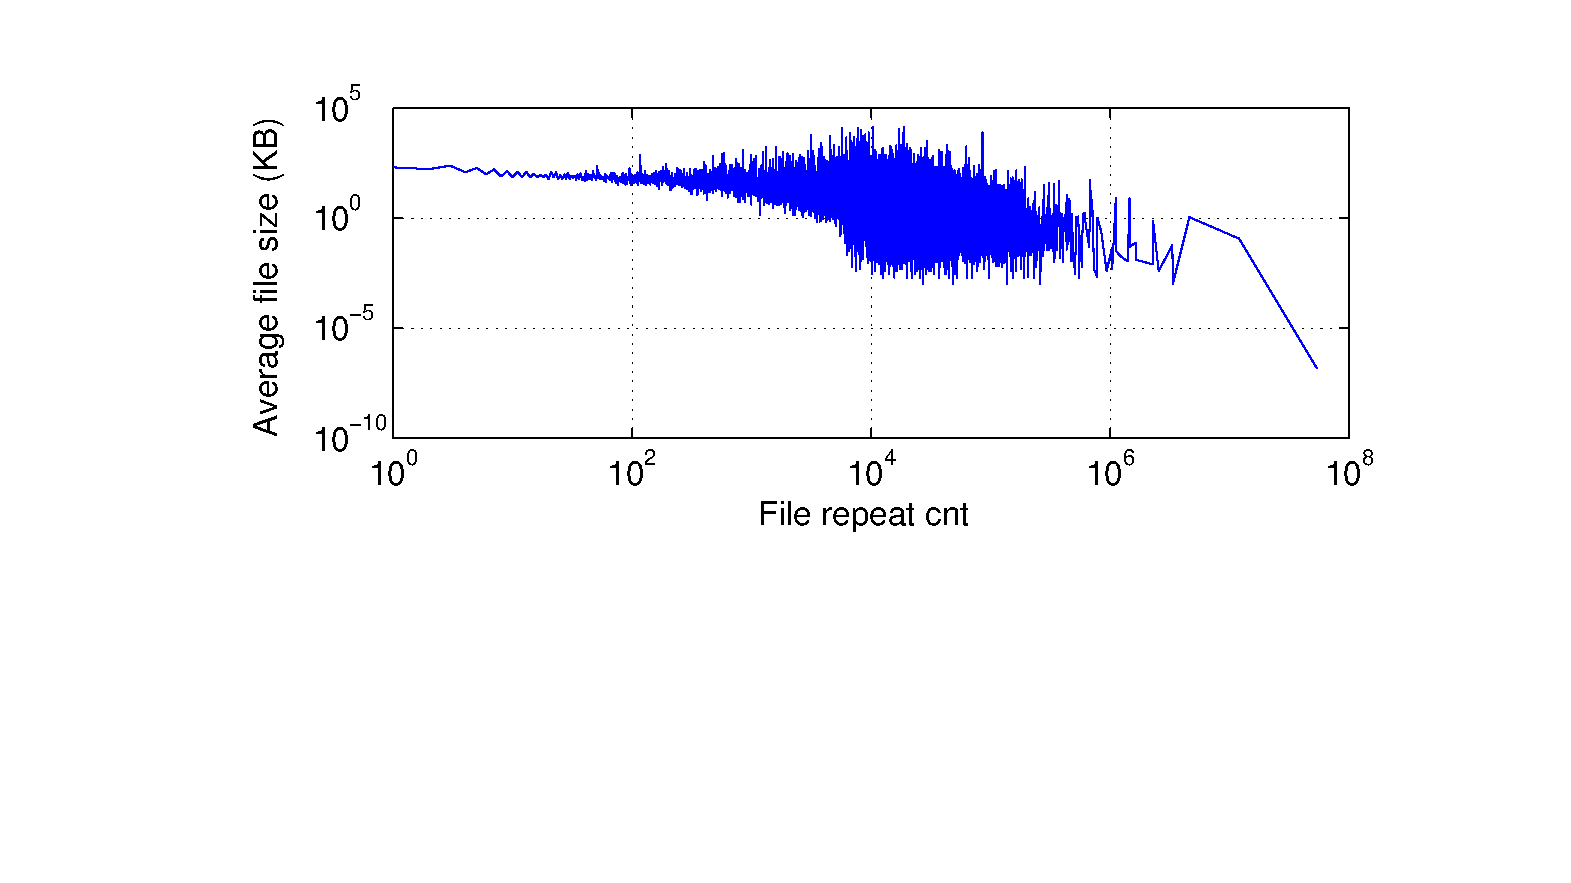
\includegraphics[width=0.5\textwidth]{graphs/avg_size_by_cnt.eps} %
%%\caption{Average file size with same repeat count.  %	} %
%%\label{fig_avg_size_by_cnt} %\end{figure} % %\paragraph{Redundant ratio by
%%file size for the files with the same content in terms of file count and
%%storage capacity} %Total size of redundant files with same content(TRS) %
%%%97\% of the TRSs are equal or less than 100MB.  % %\begin{figure} %
%%\centering %
%%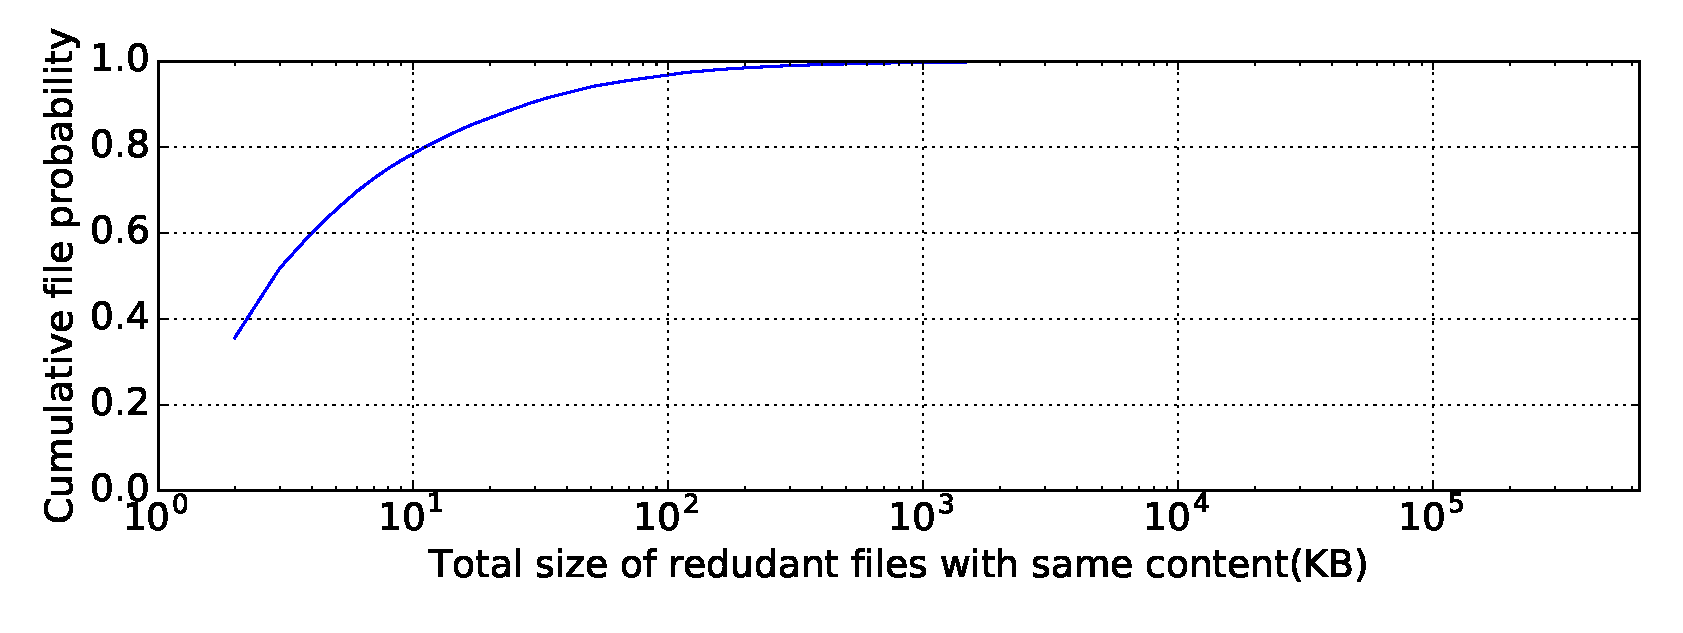
\includegraphics[width=0.5\textwidth]{graphs/Total_size_of_redudant_files_with_same_content-KB.eps}
%%%	\caption{CDF of total file size with same file content (MB).  %	} %
%%\label{fig_total_redundant_same_digest} %\end{figure} % %\paragraph{Redundant
%%ratio by repeat count for the files with the same repeat count in terms of
%%file count and storage capacity} % %However, with the increase of file repeat
%%count, the sum of file size with same repeat count becomes smaller.  %
%%%\begin{figure} %	\centering %
%%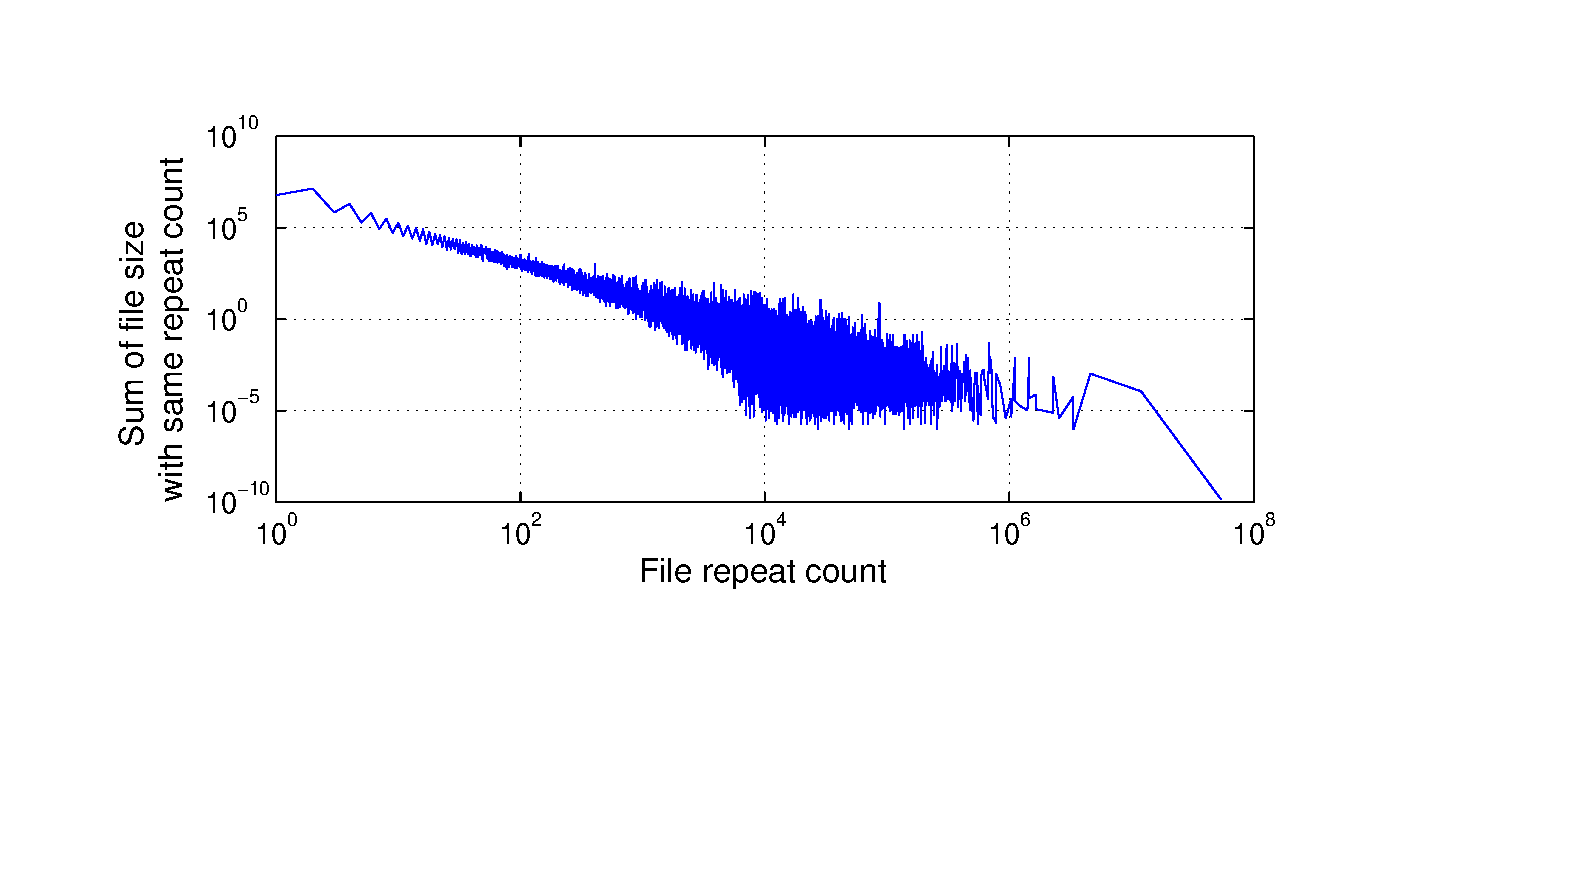
\includegraphics[width=0.5\textwidth]{graphs/sum_size_by_cnt.eps} %
%%\caption{Sum of file size with same repeat count.  %	} %
%%\label{fig_sum_by_cnt} %\end{figure}
%%
%%% %\paragraph{Cumulative distribution and probability distribution of file
%%repeat count} %\begin{table} %	\centering %	\scriptsize  %
%%%\begin{minipage}{.5\linewidth} %	\caption{Summary of image types}
%%\label{tbl:redundant_ratio} %	\begin{tabular}{|l|l|l|}%p{0.14\textwidth} %
%%\hline %		% after \\: \hline or \cline{col1-col2}
%%\cline{col3-col4} ...  %		% after \\: \hline or \cline{col1-col2}
%%\cline{col3-col4} ...  %		Image types & num. & avg. redundant
%%ratio  \\ %		\hline %		  &   &        \\ %
%%\hline %		  &   &         \\ %		\hline %
%%&   &       \\ %		   \hline %		other     &   &
%%\\ %		\hline %	\end{tabular} %\end{table}
%%
%%%\subsection{Redundant files with same filename and relative path} %
%%%\subsection{Common directories that contains redundant files} %
%%%\subsection{Redundant tar files} %\begin{table} %	\centering %
%%\scriptsize  %	%\begin{minipage}{.5\linewidth} %	\caption{Summary of
%%file \& dir. characterization} \label{tbl:sum_file_dir_char} %
%%\begin{tabular}{|l|l|l|l|l|}%p{0.14\textwidth} %		\hline %
%%% after \\: \hline or \cline{col1-col2} \cline{col3-col4} ...  %
%%% after \\: \hline or \cline{col1-col2} \cline{col3-col4} ...  %
%%Metrics & max & min & median & avg.\\ %		\hline %
%%File size &   &   &   &  \\ %		\hline %		File size
%%(repeat cnt. $>$ 1) &   &   &    &  \\ %		\hline %
%%File size (repeat cnt. $=$ 1) &   &   &    &  \\ %		\hline %
%%\hline %		Dir. size &  &  & & \\ %		\hline %
%%File cnt. per dir & &  &  & \\ %		\hline %
%%Redundant ratio & &  &  & \\ %		\hline %		Dir. depth  &
%%&  & & \\ %		\hline %	\end{tabular} %\end{table} 

